% ==============================================================================
% DOCUMENTO PRINCIPAL - LATEX
% Asignatura: Ingeniería de Software I - UNSAAC
% Laboratorio N° 05: Estimación de Esfuerzo con Planning Poker
% Proyecto: Sistema Integral de Gestión de Capacitaciones (SIGC-CUSCO)
% Autores: Choquenaira Quispe, Yaranga Achahui, Ccama Enriquez
% Docente: Ing. Lisha Sabah Diaz Caceres
% ==============================================================================

\documentclass[11pt,a4paper]{article}

% ==============================================================================
% CONFIGURACIÓN DE PAQUETES Y ESTILOS - LATEX
% UNSAAC | Asignatura: Ingeniería de Software I
% Laboratorio N° 05: Estimación de Esfuerzo con Planning Poker
% Proyecto: Sistema Integral de Gestión de Capacitaciones (SIGC-CUSCO)
% ==============================================================================

\usepackage[utf8]{inputenc}
\usepackage[T1]{fontenc}
\usepackage[spanish, es-tabla, es-nodecimaldot]{babel}
\spanishdeactivate{"}
\usepackage{csquotes}

\usepackage[margin=2.2cm, top=2.5cm, bottom=2.5cm, headheight=18pt]{geometry}

\usepackage{mathptmx}
\usepackage{setspace}
\setstretch{1.15}

\usepackage{graphicx}
\graphicspath{{./}{imagenes/}{./imagenes/}}
\usepackage{float}
\usepackage{booktabs}
\usepackage{tabularx}
\usepackage{array}
\usepackage{multirow}
\usepackage{caption}
\captionsetup{font=small, labelfont=bf, skip=6pt}

\usepackage[table]{xcolor}

\usepackage{enumitem}
\setlist{topsep=2pt, itemsep=2pt, parsep=0pt}

\usepackage{fancyhdr}
\pagestyle{fancy}
\fancyhf{}
\fancyhead[L]{\small\itshape UNSAAC -- Ingeniería de Software I}
\fancyhead[R]{\small\itshape Lab 05: Planning Poker -- SIGC-CUSCO}
\fancyfoot[C]{\thepage}
\renewcommand{\headrulewidth}{0.4pt}
\renewcommand{\footrulewidth}{0pt}

\usepackage{xurl}
\usepackage{hyperref}
\hypersetup{
    colorlinks=true,
    breaklinks=true,
    linkcolor=blue!75!black,
    urlcolor=blue!75!black,
    citecolor=blue!75!black,
    pdftitle={Lab 05 - Estimación de Esfuerzo con Planning Poker - SIGC-CUSCO},
    pdfauthor={Choquenaira, Yaranga, Ccama}
}

\usepackage{microtype}
\emergencystretch=2.5em

\setlength{\parindent}{0.6cm}
\setlength{\parskip}{0.28em}

% Tipos de columnas convenientes para tablas de requerimientos y backlog
\newcolumntype{Y}{>{\raggedright\arraybackslash}X}
\newcolumntype{P}[1]{>{\raggedright\arraybackslash}p{#1}}
\newcolumntype{C}[1]{>{\centering\arraybackslash}p{#1}}

% Colores institucionales y de clasificación ágil
\definecolor{headerblue}{RGB}{20, 65, 110}
\definecolor{rowalt}{RGB}{248, 250, 252}
\definecolor{cortaGreen}{RGB}{220, 245, 230}
\definecolor{cortaText}{RGB}{22, 101, 52}
\definecolor{mediaOrange}{RGB}{254, 243, 199}
\definecolor{mediaText}{RGB}{180, 83, 9}
\definecolor{complejaRed}{RGB}{254, 226, 226}
\definecolor{complejaText}{RGB}{185, 28, 28}

% Comandos auxiliares para etiquetas visuales de tamaño
\newcommand{\badgeCorta}{\colorbox{cortaGreen}{\textcolor{cortaText}{\textbf{\scriptsize CORTA (1--3)}}}}
\newcommand{\badgeMedia}{\colorbox{mediaOrange}{\textcolor{mediaText}{\textbf{\scriptsize MEDIA (5--8)}}}}
\newcommand{\badgeCompleja}{\colorbox{complejaRed}{\textcolor{complejaText}{\textbf{\scriptsize COMPLEJA (13+)}}}}


\begin{document}
\hypersetup{pageanchor=false}

% 1. Portada Institucional Oficial
\begin{titlepage}
    \centering
    \vspace*{0.2cm}
    
    {\fontsize{13}{16}\selectfont \textbf{UNIVERSIDAD NACIONAL DE SAN ANTONIO ABAD DEL CUSCO}}\\[0.25cm]
    {\fontsize{11}{14}\selectfont \textbf{FACULTAD DE INGENIERÍA ELÉCTRICA, ELECTRÓNICA, INFORMÁTICA Y MECÁNICA}}\\[0.25cm]
    {\fontsize{11}{14}\selectfont \textbf{ESCUELA PROFESIONAL DE INGENIERÍA INFORMÁTICA Y DE SISTEMAS}}\\[0.5cm]
    
    
\includegraphics[width=3.5cm]{escudo.png}\\[0.5cm]
    
    {\fontsize{13}{16}\selectfont \textbf{LABORATORIO N° 05}}\\[0.15cm]
    {\fontsize{12}{15}\selectfont \textbf{ESTIMACIÓN DE ESFUERZO CON PLANNING POKER}}\\[0.25cm]
    \rule{\textwidth}{1.2pt}\\[0.2cm]
    {\fontsize{13}{16.5}\selectfont \textbf{``SISTEMA INTEGRAL DE GESTIÓN DE CAPACITACIONES (SIGC-CUSCO)''}}\\[0.15cm]
    \rule{\textwidth}{1.2pt}\\[0.5cm]
    
    \begin{minipage}{0.92\textwidth}
        \setstretch{1.2}
        \textbf{Asignatura:} Ingeniería de Software I\\[0.2cm]
        \textbf{Docente:} Ing. Lisha Sabah Diaz Caceres\\[0.2cm]
        \textbf{Integrantes:}\\[0.15cm]
        \hspace*{0.4cm}\textbullet\quad Choquenaira Quispe, Noe Franklin \hfill 133962\\[0.12cm]
        \hspace*{0.4cm}\textbullet\quad Yaranga Achahui, Aldo \hfill 103179\\[0.12cm]
        \hspace*{0.4cm}\textbullet\quad Ccama Enriquez, Carolay \hfill 210921
    \end{minipage}\\[0.8cm]
    
    \vfill
    {\textbf{Cusco -- 2026}}\\[0.2cm]
\end{titlepage}


% 2. Tabla de Contenidos
\newpage
\hypersetup{pageanchor=true}
\pagenumbering{roman}
{
    \hypersetup{linkcolor=black}
    \begin{spacing}{0.95}
    \tableofcontents
    \end{spacing}
}
\newpage
\pagenumbering{arabic}

% 3. Objetivo y Fundamento Teórico
\section{Objetivo y Fundamento Teórico}

\subsection{Objetivo General y Específicos}

El presente laboratorio tiene como propósito estimar el esfuerzo relativo de desarrollo de las historias de usuario pertenecientes al \textbf{Sistema Integral de Gestión de Capacitaciones (SIGC-CUSCO)}, formuladas durante el Laboratorio 03, mediante la técnica colaborativa ágil \textbf{Planning Poker} y el empleo de \textbf{Story Points} (puntos de historia). Asimismo, se busca institucionalizar el registro y clasificación del backlog dentro de la plataforma de gestión \textbf{Jira Software}, preparando el terreno para la planificación efectiva de los sprints del proyecto.

Para cumplir con este objetivo general, se desarrollaron los siguientes objetivos específicos:
\begin{itemize}
    \item \textbf{Auditar y clarificar el Product Backlog:} Revisar minuciosamente las historias de usuario provenientes del Laboratorio 03, verificando la consistencia de su estructura (\textit{Como / Quiero / Para}) y la completitud de sus criterios de aceptación en formato BDD (\textit{Dado / Cuando / Entonces}) antes de someterlas a votación.
    \item \textbf{Establecer una historia de referencia (\textit{Golden Story}):} Identificar una historia conocida y de bajo riesgo técnico que actúe como unidad patrón de comparación relativa para calibrar las estimaciones del equipo.
    \item \textbf{Ejecutar la dinámica de Planning Poker:} Realizar una sesión de estimación con los tres integrantes del equipo de desarrollo, utilizando la escala modificada de Fibonacci, contrastando posturas técnicas divergentes y alcanzando consensos genuinos sin imposiciones jerárquicas.
    \item \textbf{Registrar y clasificar el backlog en Jira:} Cargar los valores de Story Points acordados en el proyecto \texttt{SC} de Jira Software, clasificando las historias según su tamaño en tres grupos: \textit{Cortas} (1--3 SP), \textit{Medias} (5--8 SP) y \textit{Complejas} (13+ SP).
    \item \textbf{Refinar historias sobredimensionadas (Trabajo extra):} Descomponer las historias catalogadas como complejas ($\ge 13$ SP) en historias de usuario hijas más pequeñas, atómicas y estimables ($\le 8$ SP), mitigando la incertidumbre arquitectónica mediante la formulación de spikes de investigación técnica.
\end{itemize}

\subsection{Fundamento Teórico}

\subsubsection{Estimación ágil vs. estimación tradicional en horas}
En el desarrollo de software convencional, la estimación suele abordarse asignando horas-hombre absolutas a cada tarea. La experiencia empírica y la literatura de ingeniería de software demuestran que este enfoque adolece de múltiples sesgos cognitivos:
\begin{enumerate}
    \item \textbf{Sesgo del optimismo:} Los desarrolladores tienden a estimar asumiendo un escenario ideal, ignorando interrupciones, depuración de dependencias, integración continua o tiempos de prueba.
    \item \textbf{Variabilidad individual de velocidad:} Una tarea que a un programador experimentado le toma 4 horas puede demandar 16 horas a un desarrollador junior; por tanto, el tiempo en horas no mide la magnitud intrínseca del problema.
    \item \textbf{Ley de Parkinson:} El trabajo tiende a expandirse hasta ocupar todo el tiempo asignado para su realización.
\end{enumerate}

La estimación ágil resuelve esta problemática trasladando el foco de la \textit{duración absoluta} al \textit{tamaño relativo}. La mente humana posee una notable precisión innata para comparar tamaños relativos (por ejemplo, determinar si un edificio es el doble de alto que una casa) en contraste con la dificultad de predecir la altura exacta en metros a simple vista. Al estimar historias de usuario de forma relativa frente a una historia de referencia, el equipo logra evaluaciones más rápidas, consistentes y desprovistas de compromisos temporales prematuros.

\subsubsection{Story Points (Puntos de Historia)}
Un \textbf{Story Point} es una unidad métrica abstracta que resume holísticamente tres componentes fundamentales de una historia de usuario:
\begin{itemize}
    \item \textbf{Complejidad:} Dificultad algorítmica y técnica requerida para materializar los criterios de aceptación (lógica de negocio cruzada, transacciones atómicas, validaciones de seguridad, integración de APIs de terceros o procesamiento de documentos).
    \item \textbf{Esfuerzo:} Cantidad de trabajo volumétrico necesario (número de interfaces de usuario a diseñar en Blade/Tailwind, controladores y servicios a implementar, migraciones de base de datos, semillas de prueba y pruebas automatizadas).
    \item \textbf{Incertidumbre o Riesgo:} Nivel de desconocimiento sobre la tecnología, ambigüedad en los requerimientos del cliente o riesgo de dependencias no controladas (como el comportamiento en entornos sin conectividad o la integración con pasarelas externas).
\end{itemize}

\subsubsection{Técnica Planning Poker}
El \textbf{Planning Poker} es un procedimiento de estimación colaborativo fundamentado en el método \textit{Wideband Delphi}. Diseñado específicamente para entornos ágiles (Scrum/Kanban), persigue anular dos de los problemas más frecuentes en las reuniones de equipo:
\begin{itemize}
    \item \textbf{El efecto de anclaje (\textit{Anchoring effect}):} Ocurre cuando la primera persona en expresar una cifra condiciona inconscientemente las estimaciones de los demás participantes.
    \item \textbf{La presión por conformidad o jerarquía:} La inclinación natural a subordinar la propia opinión técnica frente a integrantes con mayor antigüedad o autoridad percibida.
\end{itemize}

Para neutralizar estos efectos, la dinámica exige que todos los participantes seleccionen su voto en privado. Cuando todos han elegido, las cartas se revelan en simultáneo. Si existe dispersión en los valores, se otorga la palabra a los participantes que emitieron los votos extremos (el más alto y el más bajo) para que expongan sus argumentos técnicos, supuestos arquitectónicos o riesgos identificados. Tras un debate breve y enfocado, se procede a una nueva ronda de votación hasta alcanzar el consenso del equipo.

\subsubsection{Escala modificada de Fibonacci}
El equipo adoptó la secuencia estándar de Fibonacci:
\[
    \mathcal{F} = \{1,\, 2,\, 3,\, 5,\, 8,\, 13,\, 21\}
\]
El espaciamiento no lineal y progresivamente exponencial entre los valores refleja el \textit{Principio de Incertidumbre} en la ingeniería de software: a medida que el tamaño de un ítem se incrementa, la capacidad para predecir su costo con exactitud decae notablemente. No tiene valor práctico discernir si una funcionalidad demanda 14 o 15 puntos; en cambio, contrastar entre 13 y 21 puntos obliga al equipo a reflexionar si la tarea es simplemente grande o si oculta un riesgo técnico inaceptable que exige refinamiento inmediato.

\subsection{Herramientas Empleadas}

Para la ejecución sistemática del laboratorio se integraron las siguientes herramientas:
\begin{itemize}
    \item \textbf{Planning Poker digital:} Aplicación interactiva configurada con la baraja Fibonacci, empleada durante la sesión para la votación síncrona en tiempo real. Los registros de cada ronda y sus argumentos fueron exportados en formato estructurado a \texttt{backlog/sesion\_planning\_poker.json}.
    \item \textbf{Jira Software Cloud (Proyecto \texttt{SC} -- SIGC-CUSCO):} Plataforma principal de gestión ágil. Se habilitó el campo numérico nativo \texttt{Story point estimate}, se etiquetaron las historias (\texttt{sp-corta}, \texttt{sp-media}, \texttt{sp-compleja}, \texttt{dividida}, \texttt{refinamiento}, \texttt{lab05}) y se categorizaron conforme a las prioridades MoSCoW del sistema.
    \item \textbf{Repositorio en GitHub (\texttt{frankich99/LABO-SIGC-CUSCO}):} Repositorio institucional donde se almacena el historial de versiones del proyecto, incluyendo el backlog estimado en CSV (\texttt{backlog/product\_backlog\_estimado.csv}), las capturas de auditoría y los fuentes en \LaTeX{}.
\end{itemize}

\vspace{0.3cm}

% 4. Parte 1: Preparación del Backlog
\section{Parte 1: Preparación del Backlog}

\subsection{Revisión y Consolidación de las Historias del Lab 03}

Antes de iniciar la estimación, el equipo realizó una sesión preliminar de auditoría técnica sobre el repositorio de requerimientos elaborado en el Laboratorio 03 (\texttt{lab03/docs/jira/jira\_import\_sigc\_cusco.csv}) y su correspondiente estado en el proyecto de Jira Software. Con el objetivo de garantizar que la sesión de Planning Poker fuera ágil y careciera de ambigüedades semánticas, se ejecutaron las siguientes acciones de preparación:

\begin{enumerate}
    \item \textbf{Unificación y trazabilidad de nomenclatura en Jira:} Al cotejar el backlog con Jira, se advirtió que tres historias clave del Lab 03 habían sido registradas previamente con títulos genéricos y sin su código identificador formal. Se procedió a actualizar su resumen (\textit{Summary}) anteponiendo el código \texttt{HU-XX}:
    \begin{itemize}
        \item \textbf{SC-13:} Registrada inicialmente como \enquote{Gestionar usuarios y roles}, se homologó como \textbf{HU-10: Asignar roles a los usuarios para controlar el acceso}.
        \item \textbf{SC-14:} Registrada como \enquote{Registrar institución con logo}, se homologó como \textbf{HU-07: Registrar diferentes instituciones en el sistema}.
        \item \textbf{SC-16:} Registrada como \enquote{Crear capacitación}, se homologó como \textbf{HU-06: Crear capacitaciones con fechas, cupos y docente asignado}.
    \end{itemize}
    Las nueve historias restantes (SC-19 a SC-27) fueron sincronizadas rigurosamente en Jira manteniendo la correspondencia biunívoca con las especificaciones del Lab 03.
    
    \item \textbf{Incorporación formal de la historia de autenticación (HU-13):} En el backlog operativo de Jira existía el issue \textbf{SC-18: Iniciar sesión con DNI y recuperar contraseña}, fundamental para el acceso al sistema pero que no contaba con código \texttt{HU} en el archivo plano inicial. Para no dejar fuera del dimensionamiento este flujo crítico, el equipo la formalizó como \textbf{HU-13}, alcanzando un total de 13 historias candidatas para la sesión.
    
    \item \textbf{Vinculación a Épicas de producto:} Cada historia fue enlazada en Jira con su respectiva Épica funcional para facilitar el análisis del esfuerzo por subsistema:
    \begin{itemize}
        \item \textbf{SC-7:} Gestión Multientidad y Usuarios (\texttt{HU-07}, \texttt{HU-10}, \texttt{HU-13}).
        \item \textbf{SC-8:} Catálogo e Inscripción (\texttt{HU-01}, \texttt{HU-06}, \texttt{HU-12}).
        \item \textbf{SC-9:} Control de Asistencia Digital (QR) (\texttt{HU-03}, \texttt{HU-11}).
        \item \textbf{SC-10:} Registro Académico y Evaluación (\texttt{HU-04}).
        \item \textbf{SC-11:} Certificados con Verificación QR (\texttt{HU-05}, \texttt{HU-08}).
        \item \textbf{SC-12:} Reportes y Notificaciones (\texttt{HU-02}, \texttt{HU-09}).
    \end{itemize}
    
    \item \textbf{Aclaración previa de alcance y criterios de aceptación:} El equipo revisó que cada tarjeta contara con su redacción bajo la estructura \textit{Como / Quiero / Para} y con sus criterios de aceptación redactados en formato BDD (\textit{Dado / Cuando / Entonces}). Durante la revisión se aclararon dudas sobre el alcance que en iteraciones anteriores generaban confusión, como por ejemplo si la emisión de certificados en \texttt{HU-05} contemplaba la generación masiva o solo individual, o si la multientidad de \texttt{HU-07} exigía bases de datos físicas independientes.
    
    \item \textbf{Selección de la Historia de Referencia (\textit{Golden Story}):} Como buena práctica de estimación ágil, el equipo seleccionó de mutuo acuerdo la historia \textbf{HU-12: Consultar catálogo público de cursos disponibles} como unidad patrón de calibración, asignándole de forma unánime el valor base de \textbf{3 Story Points}.
    
    \textit{Justificación técnica de la referencia:} \texttt{HU-12} comprende una consulta indexada a la base de datos de cursos con estado publicado, un listado responsive con buscador y contador de vacantes en tiempo real, sin requerir sesión iniciada ni mutaciones transaccionales complejas. Dicha funcionalidad es perfectamente dominada por los integrantes, convirtiéndose en el patrón métrico: las historias más simples se estimarían en 1 o 2 SP, mientras que aquellas con mayor lógica transaccional, seguridad o incertidumbre escalarían a 5, 8, 13 o 21 SP.
\end{enumerate}

\subsection{Backlog Preparado para la Sesión}

La Tabla~\ref{tab:backlog_preparado} consolida las 13 historias de usuario preparadas, con su clave en Jira, código funcional, título normalizado, épica asociada y su correspondiente clasificación de prioridad MoSCoW.

\begin{table}[H]
\centering
\small
\renewcommand{\arraystretch}{1.2}
\caption{Product Backlog preparado y verificado para la sesión de Planning Poker (13 historias).}
\label{tab:backlog_preparado}
\begin{tabularx}{\textwidth}{P{1.4cm} P{1.4cm} Y P{3.8cm} C{2.6cm}}
\toprule
\rowcolor{headerblue}
\textcolor{white}{\textbf{Clave}} & \textcolor{white}{\textbf{Código}} & \textcolor{white}{\textbf{Historia de Usuario}} & \textcolor{white}{\textbf{Épica Asociada}} & \textcolor{white}{\textbf{Prioridad MoSCoW}} \\
\midrule
\rowcolor{white}
SC-13 & HU-10 & Asignar roles a los usuarios para controlar el acceso & Multientidad y Usuarios & Highest / Must \\
\rowcolor{rowalt}
SC-16 & HU-06 & Crear capacitaciones con fechas, cupos y docente & Catálogo e Inscripción & Highest / Must \\
\rowcolor{white}
SC-19 & HU-01 & Inscribirme a una capacitación usando mi DNI & Catálogo e Inscripción & Highest / Must \\
\rowcolor{rowalt}
SC-20 & HU-03 & Pasar asistencia escaneando un código QR & Control de Asistencia QR & High / Must \\
\rowcolor{white}
SC-21 & HU-04 & Registrar notas y calcular aprobación automáticamente & Evaluación y Actas & High / Must \\
\rowcolor{rowalt}
SC-22 & HU-05 & Generar y descargar certificado PDF con código QR & Certificados con QR & High / Must \\
\rowcolor{white}
SC-14 & HU-07 & Registrar diferentes instituciones en el sistema & Multientidad y Usuarios & Medium / Should \\
\rowcolor{rowalt}
SC-23 & HU-08 & Verificar autenticidad de certificado mediante QR & Certificados con QR & Medium / Should \\
\rowcolor{white}
SC-24 & HU-09 & Generar reportes de capacitaciones para auditorías & Reportes y Notificaciones & Medium / Should \\
\rowcolor{rowalt}
SC-25 & HU-02 & Recibir correo de confirmación al inscribirme & Reportes y Notificaciones & Medium / Should \\
\rowcolor{white}
SC-18 & HU-13 & Iniciar sesión con DNI y recuperar contraseña & Multientidad y Usuarios & Medium / Should \\
\rowcolor{rowalt}
SC-26 & HU-12 & Consultar catálogo público de cursos disponibles & Catálogo e Inscripción & Low / Could \textit{(Ref.)} \\
\rowcolor{white}
SC-27 & HU-11 & Marcar asistencia en modo offline con sincronización & Control de Asistencia QR & Low / Could \\
\bottomrule
\end{tabularx}
\end{table}

\vspace{0.3cm}

% 5. Parte 2: Sesión de Planning Poker y Consenso
\section{Parte 2: Sesión de Planning Poker}

\subsection{Dinámica de la Sesión en el Laboratorio}

La sesión de Planning Poker se llevó a cabo de manera presencial entre los tres integrantes del equipo de desarrollo: \textbf{Noe Franklin Choquenaira Quispe}, \textbf{Aldo Yaranga Achahui} y \textbf{Carolay Ccama Enriquez}. Para garantizar el rigor metodológico exigido por la guía de laboratorio, se siguió estrictamente el protocolo de cinco pasos para cada una de las 13 historias de usuario:

\begin{enumerate}
    \item \textbf{Selección y lectura de la historia:} Siguiendo el orden de prioridad MoSCoW, se leyó en voz alta la historia de usuario junto con sus criterios de aceptación. El Product Owner aclaró el alcance funcional esperado.
    \item \textbf{Asignación secreta del valor:} Cada integrante seleccionó en privado su estimación en la baraja digital de Fibonacci ($1, 2, 3, 5, 8, 13, 21$), evaluando mentalmente el esfuerzo, la complejidad algorítmica y la incertidumbre técnica frente a la historia de referencia (\texttt{HU-12} = 3 SP).
    \item \textbf{Revelación simultánea y comparación:} A la cuenta de tres, todos los integrantes revelaron sus cartas al unísono. Si los valores coincidían plenamente o distaban en solo un peldaño contiguo de la escala, se procedía a un ajuste rápido.
    \item \textbf{Discusión técnica de discrepancias:} Cuando la distancia entre votos era de dos o más posiciones en la escala Fibonacci, se abrió de inmediato el debate. El participante con el voto más alto explicó los riesgos o dificultades técnicas que vislumbraba, mientras que el participante con el voto más bajo argumentó por qué consideraba la tarea más sencilla o reutilizable.
    \item \textbf{Consenso y segunda ronda:} Tras la deliberación, se realizó una segunda ronda de votación para las historias polémicas o se formalizó el consenso unánime del valor final.
\end{enumerate}

La Figura~\ref{fig:sesion_planning_poker} exhibe el panel digital de la sesión, donde se aprecian las tarjetas con los votos individuales por ronda de cada integrante (resaltando en rojo el voto más alto y en verde el voto más bajo) y el puntaje final de consenso.

\begin{figure}[H]
    \centering
    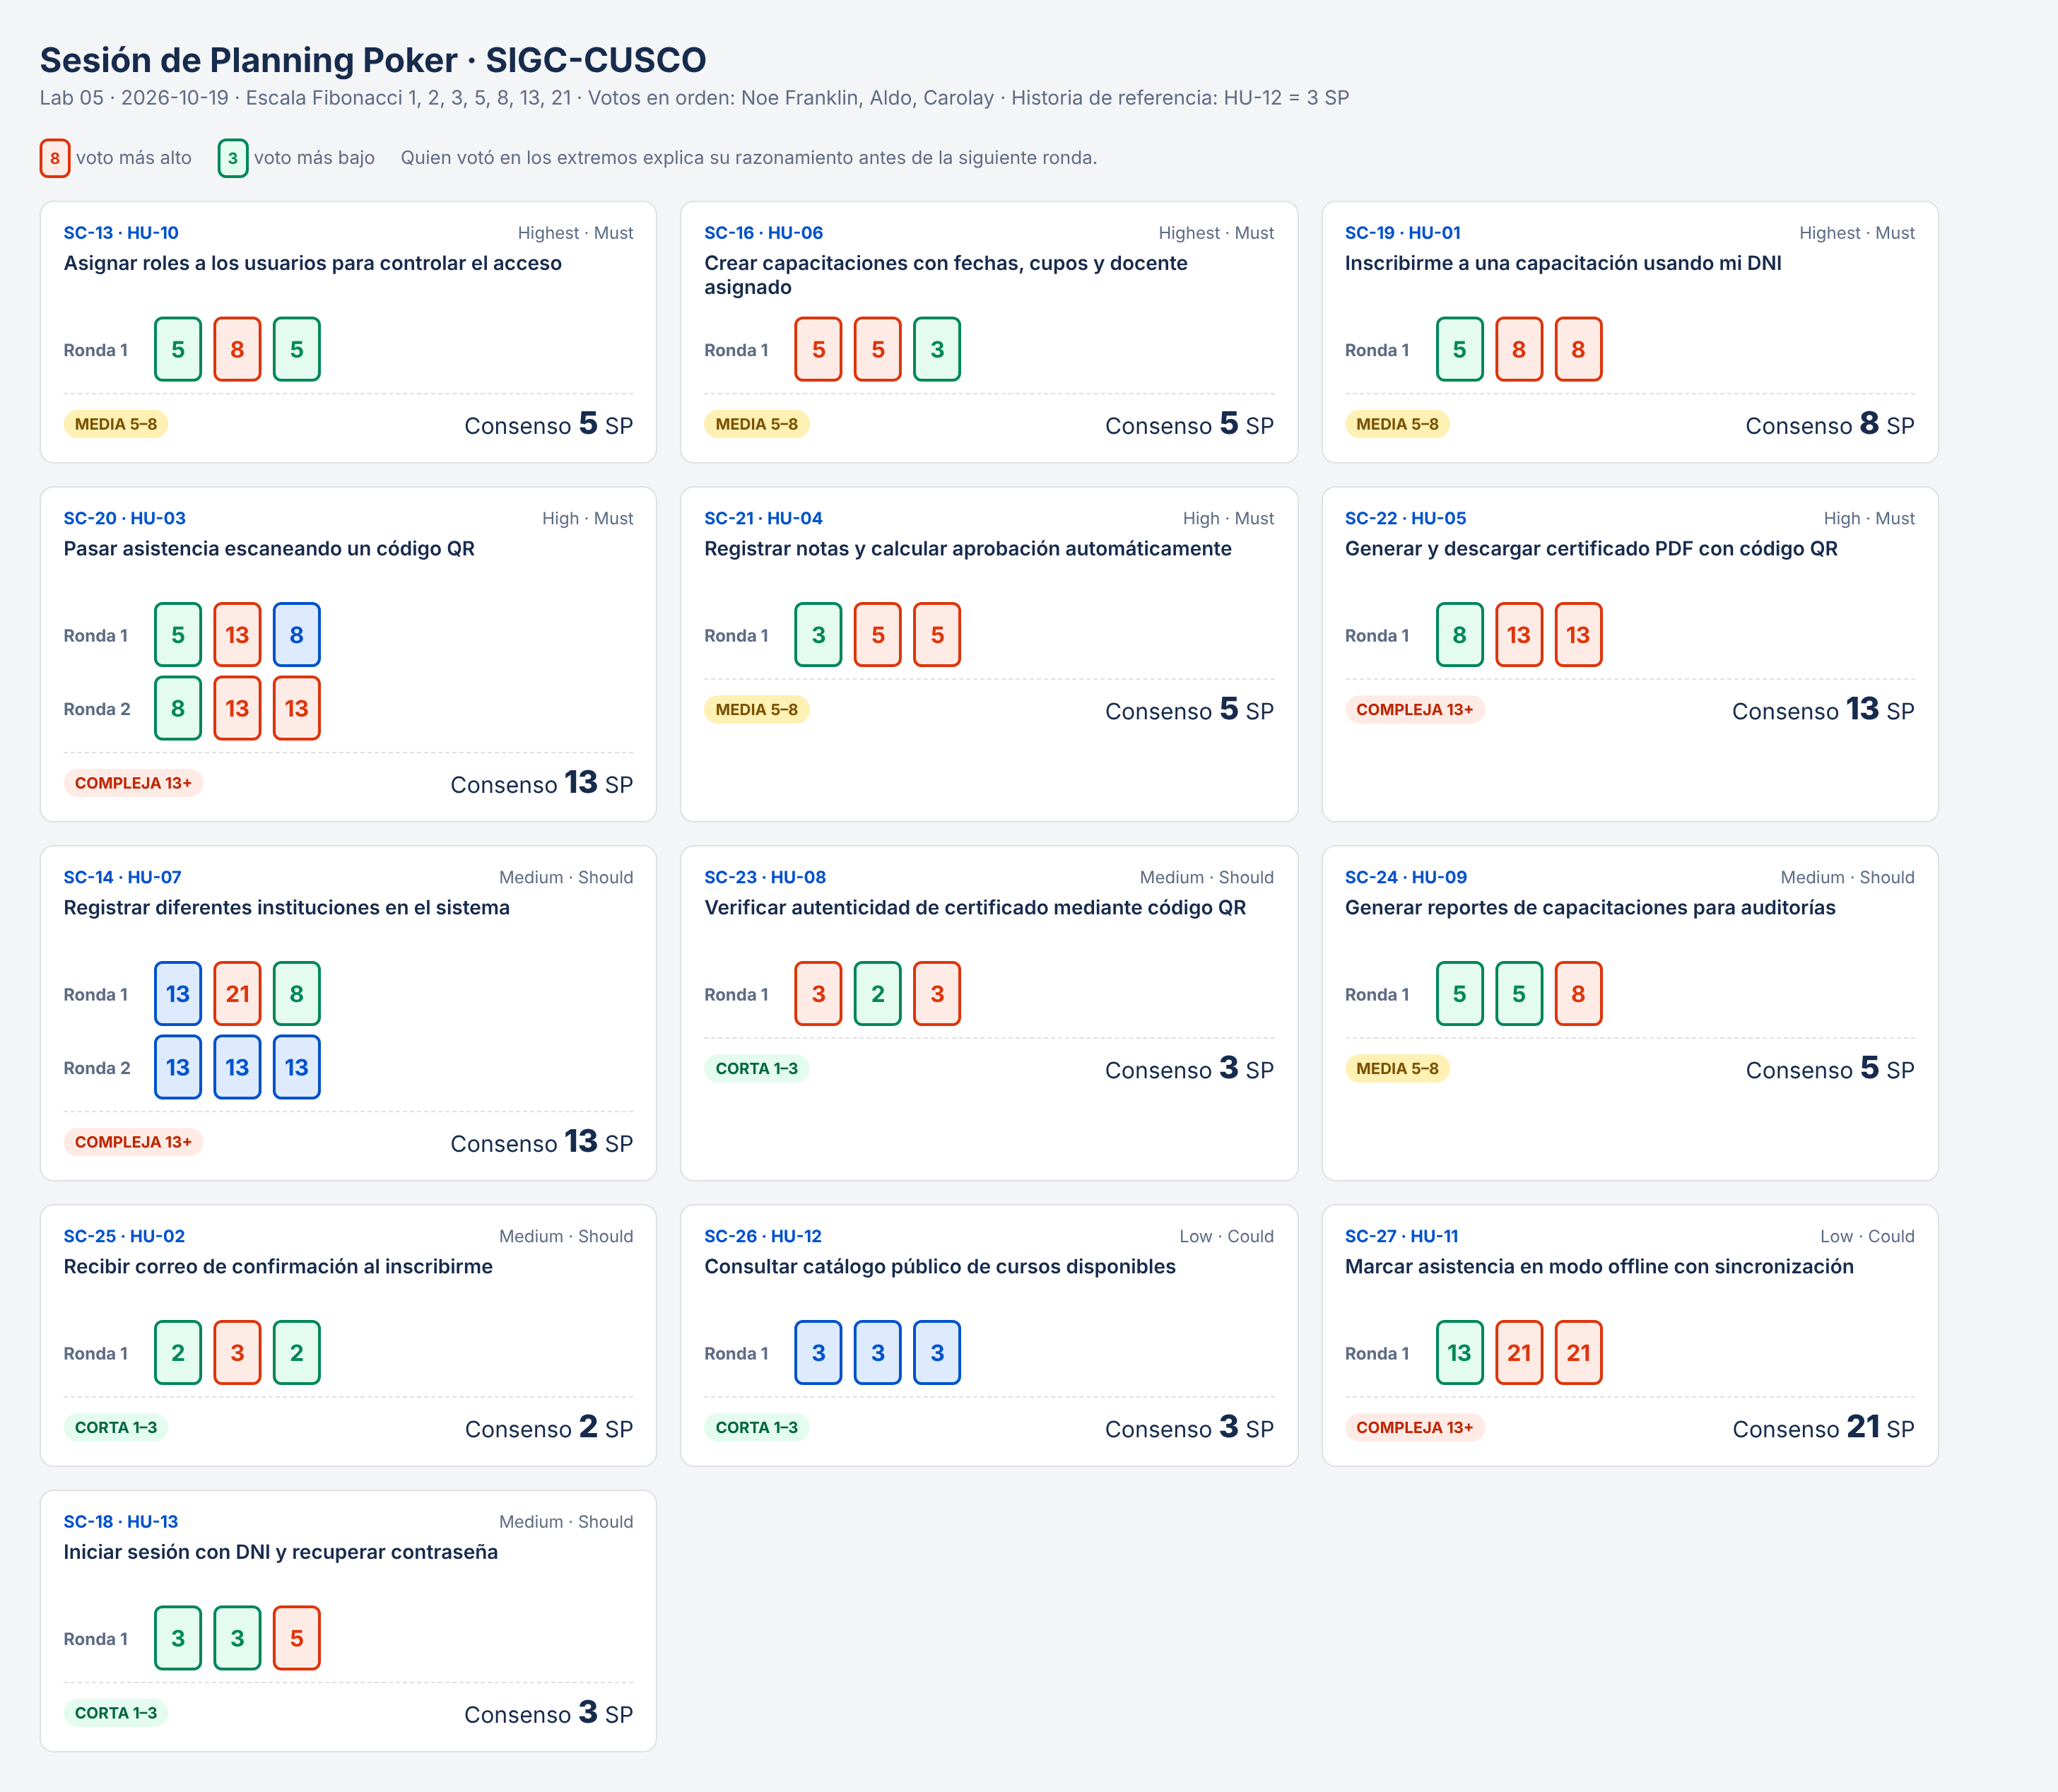
\includegraphics[width=\textwidth]{figura1_sesion_planning_poker.png}
    \caption{Evidencia gráfica de la sesión de Planning Poker: votos individuales por ronda de los tres integrantes y valor de consenso acordado por historia (rojo = voto más alto, verde = voto más bajo).}
    \label{fig:sesion_planning_poker}
\end{figure}

\subsection{Votos por Historia y Rondas de Deliberación}

En la Tabla~\ref{tab:votos_sesion} se registra el historial de votaciones obtenido durante la dinámica, mostrando las estimaciones de cada integrante en el orden cronológico de votación: \textbf{Noe Franklin / Aldo / Carolay}.

\begin{table}[H]
\centering
\small
\renewcommand{\arraystretch}{1.2}
\caption{Registro de votos individuales por ronda y consenso alcanzado (orden: Noe Franklin / Aldo / Carolay).}
\label{tab:votos_sesion}
\begin{tabularx}{\textwidth}{P{1.4cm} P{1.4cm} Y P{3.2cm} C{1.8cm}}
\toprule
\rowcolor{headerblue}
\textcolor{white}{\textbf{Clave}} & \textcolor{white}{\textbf{Código}} & \textcolor{white}{\textbf{Historia de Usuario}} & \textcolor{white}{\textbf{Votos por Ronda}} & \textcolor{white}{\textbf{Consenso SP}} \\
\midrule
\rowcolor{white}
SC-13 & HU-10 & Asignar roles a los usuarios para controlar el acceso & R1: 5 / 8 / 5 & \textbf{5 SP} \\
\rowcolor{rowalt}
SC-16 & HU-06 & Crear capacitaciones con fechas, cupos y docente asignado & R1: 5 / 5 / 3 & \textbf{5 SP} \\
\rowcolor{white}
SC-19 & HU-01 & Inscribirme a una capacitación usando mi DNI & R1: 5 / 8 / 8 & \textbf{8 SP} \\
\rowcolor{rowalt}
SC-20 & HU-03 & Pasar asistencia escaneando un código QR & R1: 5 / 13 / 8 \newline R2: 8 / 13 / 13 & \textbf{13 SP} \\
\rowcolor{white}
SC-21 & HU-04 & Registrar notas y calcular aprobación automáticamente & R1: 3 / 5 / 5 & \textbf{5 SP} \\
\rowcolor{rowalt}
SC-22 & HU-05 & Generar y descargar certificado PDF con código QR & R1: 8 / 13 / 13 & \textbf{13 SP} \\
\rowcolor{white}
SC-14 & HU-07 & Registrar diferentes instituciones en el sistema & R1: 13 / 21 / 8 \newline R2: 13 / 13 / 13 & \textbf{13 SP} \\
\rowcolor{rowalt}
SC-23 & HU-08 & Verificar autenticidad de certificado mediante código QR & R1: 3 / 2 / 3 & \textbf{3 SP} \\
\rowcolor{white}
SC-24 & HU-09 & Generar reportes de capacitaciones para auditorías & R1: 5 / 5 / 8 & \textbf{5 SP} \\
\rowcolor{rowalt}
SC-25 & HU-02 & Recibir correo de confirmación al inscribirme & R1: 2 / 3 / 2 & \textbf{2 SP} \\
\rowcolor{white}
SC-26 & HU-12 & Consultar catálogo público de cursos disponibles & R1: 3 / 3 / 3 & \textbf{3 SP} \textit{(Ref.)} \\
\rowcolor{rowalt}
SC-27 & HU-11 & Marcar asistencia en modo offline con sincronización & R1: 13 / 21 / 21 & \textbf{21 SP} \\
\rowcolor{white}
SC-18 & HU-13 & Iniciar sesión con DNI y recuperar contraseña & R1: 3 / 3 / 5 & \textbf{3 SP} \\
\bottomrule
\end{tabularx}
\end{table}

\subsection{Discusión Técnica y Argumentación del Consenso}

A continuación, se documenta la deliberación técnica suscitada en cada una de las historias de usuario, reflejando los motivos que llevaron al equipo a converger en el valor de consenso:

\begin{itemize}
    \item \textbf{HU-10: Asignar roles a los usuarios (5 SP):} En la primera ronda, Aldo votó \textbf{8} al considerar que se debía diseñar un esquema dinámico de permisos modulares granulares (matriz RBAC configurable en base de datos tipo paquete Spatie). Franklin y Carolay (ambos con voto \textbf{5}) argumentaron que el alcance para esta versión del SIGC-CUSCO requiere únicamente cuatro roles predefinidos (\textit{SuperAdmin}, \textit{Admin Entidad}, \textit{Docente} y \textit{Participante}), implementables de manera limpia mediante \textit{Gates} y \textit{Policies} nativas de Laravel. Aldo coincidió en que restringir los roles a un conjunto fijo disminuye drásticamente el esfuerzo, consolidándose el consenso en \textbf{5 SP}.
    
    \item \textbf{HU-06: Crear capacitaciones con fechas y cupos (5 SP):} Carolay emitió un voto de \textbf{3}, concibiéndola como un formulario CRUD estándar sobre la tabla de cursos. Franklin y Aldo (ambos con \textbf{5}) le hicieron notar la lógica de negocio subyacente: validación de coherencia temporal (fecha de inicio anterior a fin, fecha límite de inscripción), cruce de horarios para que un docente no sea asignado a dos capacitaciones simultáneas, y la transición automática de estados del curso (\textit{Borrador}, \textit{Abierto}, \textit{En Curso}, \textit{Finalizado}). Carolay reconoció estas restricciones de integridad y se convino \textbf{5 SP}.
    
    \item \textbf{HU-01: Inscribirme a una capacitación usando DNI (8 SP):} Franklin votó \textbf{5}, pensando únicamente en la captura del formulario de inscripción. Por el contrario, Aldo y Carolay votaron \textbf{8} señalando dos riesgos mayúsculos: la necesidad de validar el formato y dígito verificador del DNI peruano (o consumir un servicio REST de RENIEC con control de timeouts/caché) y, primordialmente, el control de concurrencia en la asignación de cupos. Para evitar sobrecupos (\textit{race conditions}) cuando varios postulantes se inscriben al mismo segundo para la última vacante, se requiere el uso de transacciones atómicas de base de datos (\texttt{DB::transaction}) con bloqueo pesimista (\texttt{lockForUpdate}). Franklin aceptó la trascendencia técnica de este riesgo y se consensuó en \textbf{8 SP}.
    
    \item \textbf{HU-03: Pasar asistencia escaneando código QR (13 SP):} Esta historia generó la mayor dispersión inicial de la jornada: Franklin votó \textbf{5}, Carolay \textbf{8} y Aldo \textbf{13}. Franklin propuso una solución elemental: proyectar un código QR estático en la pizarra del aula para que los alumnos lo escanearan con el celular. Aldo refutó inmediatamente esta idea, demostrando que un QR estático es vulnerable al fraude académico: un estudiante en el aula puede fotografiar el QR y enviarlo vía WhatsApp a compañeros ausentes para que marquen asistencia desde sus casas. Para cumplir los estándares de seguridad, el sistema debe generar un QR dinámico con token criptográfico temporal (TOTP) que expire cada 20 a 30 segundos, validando además que un participante no registre dos veces su asistencia en la misma sesión. Carolay respaldó la necesidad de robustez y, en la segunda ronda, los votos fueron \textbf{8 / 13 / 13}, acordando unánimemente \textbf{13 SP}. Por su tamaño y riesgo, fue clasificada como candidata prioritaria para refinamiento.
    
    \item \textbf{HU-04: Registrar notas y calcular aprobación automáticamente (5 SP):} Franklin votó \textbf{3}, mientras que Aldo y Carolay votaron \textbf{5}. La regla de negocio base (nota final $\ge 11$ en la escala vigesimal de 0 a 20) es sencilla; no obstante, el flujo exige una matriz interactiva de calificaciones para el docente, validación estricta de rangos y el mecanismo formal de \enquote{Cierre de Acta}, el cual debe sellar la edición de notas de manera irreversible para garantizar la inmutabilidad de los registros académicos. El equipo acordó rápidamente fijar la historia en \textbf{5 SP}.
    
    \item \textbf{HU-05: Generar y descargar certificado PDF con código QR (13 SP):} Votada con \textbf{8 / 13 / 13}. Franklin pensó que la librería \texttt{DomPDF} simplificaría todo el proceso; sin embargo, Aldo y Carolay explicaron la amplitud del alcance: se debe verificar que el alumno cumpla doble condición (nota aprobatoria $\ge 11$ y asistencia mínima al $80\%$), diseñar la maqueta visual del diploma con tipografía y escudo institucional, calcular un hash SHA-256 único antifalsificación incrustado en el documento, generar un código QR vectorial de validación y proveer la capacidad de descarga masiva para el docente. Ante la envergadura del motor de generación, Franklin aceptó el consenso en \textbf{13 SP}, programándose su refinamiento en historias más pequeñas.
    
    \item \textbf{HU-07: Registrar diferentes instituciones en el sistema (13 SP):} La primera ronda mostró una discordancia crítica: Franklin votó \textbf{13}, Aldo \textbf{21} y Carolay \textbf{8}. Carolay consideraba únicamente la interfaz administrativa para dar de alta una institución (RUC, nombre, logo). Por su parte, Aldo contemplaba el peor escenario de la arquitectura multientidad: separar los datos en esquemas o bases de datos físicas independientes, lo cual disparaba el esfuerzo a 21 SP. En la discusión se clarificó la decisión de diseño: se empleará un esquema compartido con clave foránea \texttt{institution\_id} y \textit{Global Scopes} de Eloquent en Laravel para filtrar automáticamente los registros. Esta aclaración disipó el temor de bases de datos aisladas pero mantuvo la necesidad de auditar que ningún controlador filtre información entre entidades. En la segunda ronda, la votación fue unánime: \textbf{13 / 13 / 13} (\textbf{13 SP}).
    
    \item \textbf{HU-08: Verificar autenticidad de certificado mediante QR (3 SP):} Votación expedita (Franklin \textbf{3}, Aldo \textbf{2}, Carolay \textbf{3}). Consiste en un endpoint público de solo lectura que recibe el hash o código del certificado y devuelve el estado de validez institucional. Al depender del esquema ya resuelto en \texttt{HU-05}, su complejidad es mínima. Consenso cerrado en \textbf{3 SP}.
    
    \item \textbf{HU-09: Generar reportes para auditorías (5 SP):} Carolay votó \textbf{8} anticipando exigencias complejas de auditoría gubernamental (OSCE / Contraloría). Tras deliberar, el equipo acordó estructurar una plantilla consolidada estándar en formato Excel (.xlsx) mediante la librería \texttt{PhpSpreadsheet}, con totales de inscritos, asistencias y notas. Se cerró en \textbf{5 SP}.
    
    \item \textbf{HU-02: Correo de confirmación de inscripción (2 SP):} Votación baja (Franklin \textbf{2}, Aldo \textbf{3}, Carolay \textbf{2}). El framework Laravel ya cuenta con el sistema de mensajería asíncrona (\texttt{Mailable}) y colas de trabajo (\textit{Queues}) preconfigurado; únicamente se requiere maquetar la plantilla HTML responsiva y disparar el evento tras la persistencia de la inscripción. Consenso en \textbf{2 SP}.
    
    \item \textbf{HU-12: Catálogo público de cursos (3 SP):} Historia de referencia del equipo. La votación fue unánime en primera ronda (\textbf{3 / 3 / 3}).
    
    \item \textbf{HU-11: Marcar asistencia en modo offline con sincronización (21 SP):} Votación contundente: Franklin \textbf{13}, Aldo \textbf{21} y Carolay \textbf{21}. Constituye la funcionalidad de mayor incertidumbre técnica de todo el SIGC-CUSCO. El requerimiento exige que los docentes en zonas rurales de la región Cusco (sin cobertura de internet) puedan pasar asistencia en sus dispositivos móviles y que, al recuperar la conexión, las asistencias se sincronicen bidireccionalmente sin generar duplicados ni sobrescribir registros previos. Dado que ningún integrante del equipo ha implementado previamente \textit{Service Workers}, almacenamiento en \textit{IndexedDB} y protocolos de resolución de conflictos, la incertidumbre es máxima. El equipo acordó unánimemente el techo de la escala: \textbf{21 SP}, determinando que es mandatorio aislar la tecnología mediante un spike de investigación en el trabajo extra.
    
    \item \textbf{HU-13: Iniciar sesión con DNI y recuperar contraseña (3 SP):} Votos \textbf{3 / 3 / 5}. Carolay votó 5 previendo el flujo de tokens por correo; no obstante, el kit de autenticación de Laravel resuelve nativamente el hashing de contraseñas con Bcrypt, la expiración de enlaces y las sesiones seguras, requiriendo únicamente cambiar la columna de autenticación de \texttt{email} a \texttt{dni}. Consenso en \textbf{3 SP}.
\end{itemize}

\subsection{Análisis de Dispersión y Comportamiento del Consenso}

Al analizar estadísticamente los resultados de la sesión, se constata que:
\begin{enumerate}
    \item En \textbf{10 de las 13 historias} (el $77\%$), el equipo alcanzó consenso en la primera ronda con diferencias máximas de un peldaño contiguo en Fibonacci, evidenciando un entendimiento alineado del alcance general del sistema.
    \item Únicamente en \textbf{3 historias} (\texttt{HU-03}, \texttt{HU-07} y \texttt{HU-11}) se registraron divergencias profundas ($\ge 2$ niveles de la escala). Resulta sumamente significativo que estas tres historias coincidieran con las funcionalidades de mayor incertidumbre técnica y riesgos de arquitectura (prevención de fraude en QR, aislamiento multientidad y persistencia offline).
    \item El ejercicio demostró el valor cardinal del Planning Poker: la revelación simultánea desarticuló cualquier sesgo de anclaje, y los debates técnicos sacaron a flote requisitos no funcionales críticos (concurrencia, seguridad criptográfica y manejo de estados sin red) que habrían pasado desapercibidos en una estimación individual.
\end{enumerate}

\vspace{0.3cm}

% 6. Parte 3: Registro de Estimaciones en Jira y Clasificación
\section{Parte 3: Registro de Estimaciones}

\subsection{Registro y Configuración en Jira Software}

Una vez alcanzado el consenso en la sesión de Planning Poker, se procedió a asentar los resultados dentro del proyecto oficial de Jira Software (\textbf{Proyecto \texttt{SC} -- SIGC-CUSCO}). Para garantizar la máxima trazabilidad operativa y el control visual del progreso, se configuraron los siguientes elementos en cada tarjeta:

\begin{enumerate}
    \item \textbf{Campo numérico nativo de estimación:} Se ingresó el puntaje acordado en el campo estándar \texttt{Story point estimate} de Jira, permitiendo que la plataforma calcule automáticamente la velocidad del equipo y el peso de los sprints.
    \item \textbf{Etiquetas semánticas de clasificación:} Con el objetivo de filtrar y generar vistas agrupadas de manera instantánea, se incorporaron etiquetas estandarizadas:
    \begin{itemize}
        \item Por tamaño relativo: \texttt{sp-corta}, \texttt{sp-media} y \texttt{sp-compleja}.
        \item Por alcance de práctica: \texttt{lab05}.
        \item Por prioridad de negocio: \texttt{moscow-must}, \texttt{moscow-should} y \texttt{moscow-could}.
        \item Para trazabilidad de refactorización ágil: \texttt{dividida} (para las historias padre complejas) y \texttt{refinamiento} (para las historias hijas resultantes).
    \end{itemize}
    \item \textbf{Memoria técnica de votación:} En la descripción de cada issue o en su sección de comentarios, se dejó constancia formal de las rondas de votación registradas (ej. \enquote{Ronda 1: 5 / 13 / 8, Ronda 2: 8 / 13 / 13 $\rightarrow$ Consenso 13 SP}) y la justificación técnica resumida que sustentó la decisión del equipo.
\end{enumerate}

Las Figuras~\ref{fig:jira_backlog_p1} y~\ref{fig:jira_backlog_p2} presentan la vista general del Backlog en Jira Software, donde se aprecia la distribución de las historias de usuario, sus épicas asociadas y el puntaje asignado en la columna derecha.

\begin{figure}[H]
    \centering
    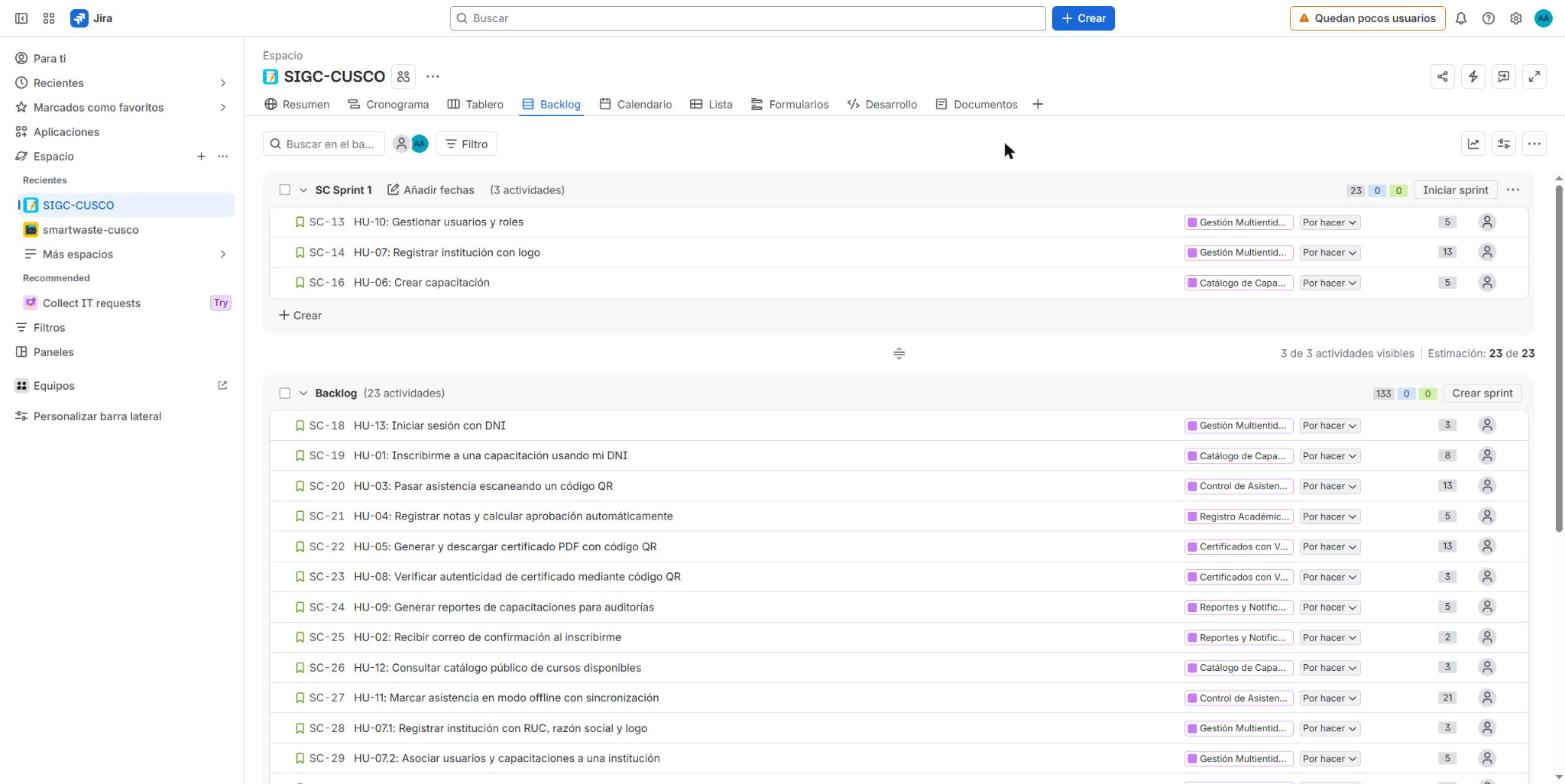
\includegraphics[width=\textwidth]{figura2_backlog_jira_parte1.jpg}
    \caption{Backlog del proyecto SC en Jira Software con la estimación en story points (columna derecha). Parte 1: SC Sprint 1 planificado y primeras historias del backlog general.}
    \label{fig:jira_backlog_p1}
\end{figure}

\begin{figure}[H]
    \centering
    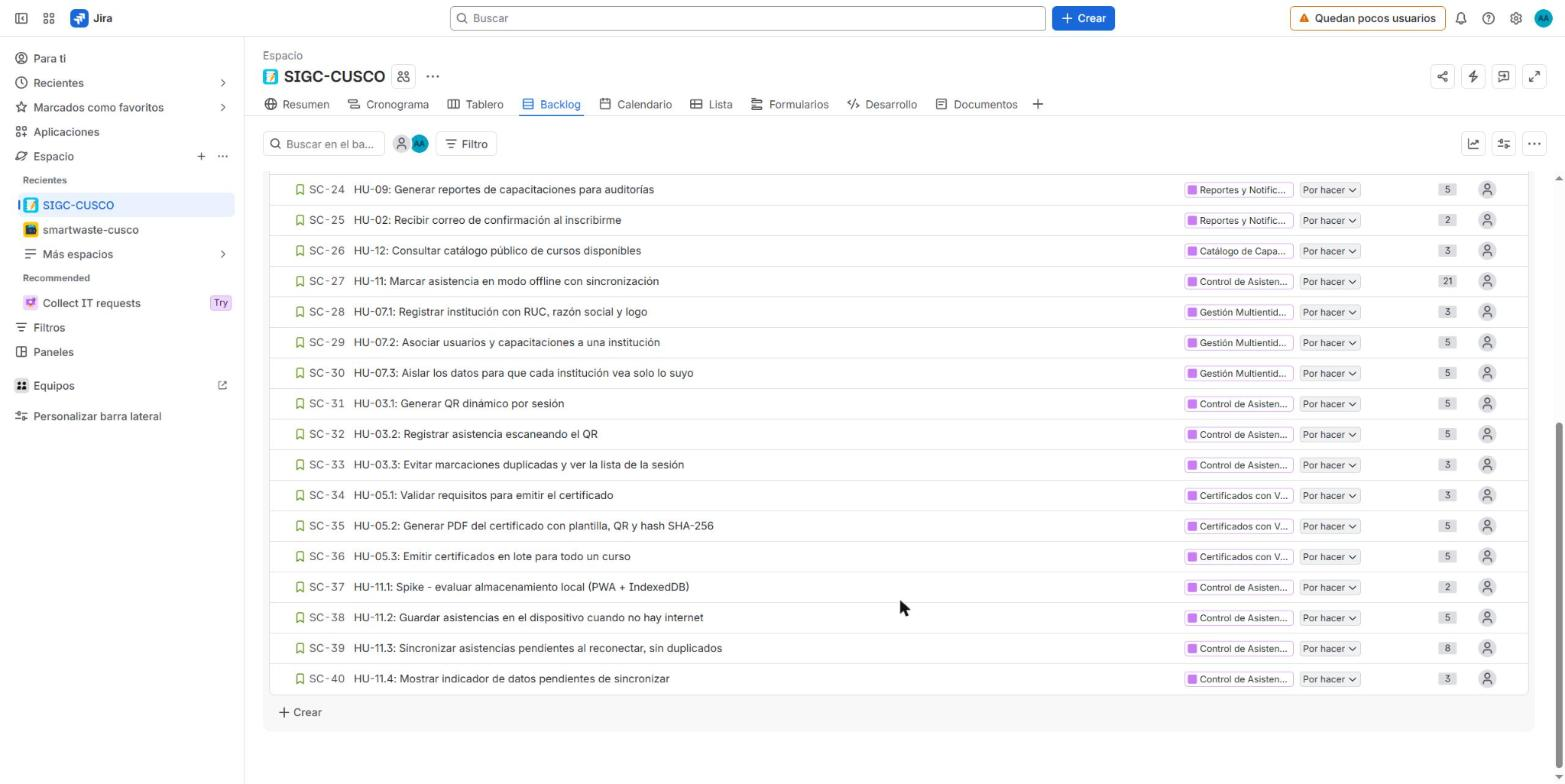
\includegraphics[width=\textwidth]{figura3_backlog_jira_parte2.jpg}
    \caption{Backlog en Jira Software, Parte 2: historias SC-24 a SC-40 (incluyendo las historias hijas refinadas). La columna de Story Points refleja la completitud del registro.}
    \label{fig:jira_backlog_p2}
\end{figure}

Para gestionar eficazmente las historias de gran envergadura que ponen en riesgo la predictibilidad de las iteraciones, se configuró el filtro de búsqueda avanzada JQL:
\begin{center}
    \texttt{project = SC AND labels = sp-compleja}
\end{center}
Dicha consulta extrae de forma inmediata los ítems que requieren descomposición obligatoria antes de ingresar al Sprint Planning. La Figura~\ref{fig:jira_detalle_sc20} muestra como ejemplo la tarjeta detallada de \textbf{SC-20 (HU-03)}, exhibiendo sus criterios de aceptación en formato BDD, el historial de votos documentado y las etiquetas asignadas.

\begin{figure}[H]
    \centering
    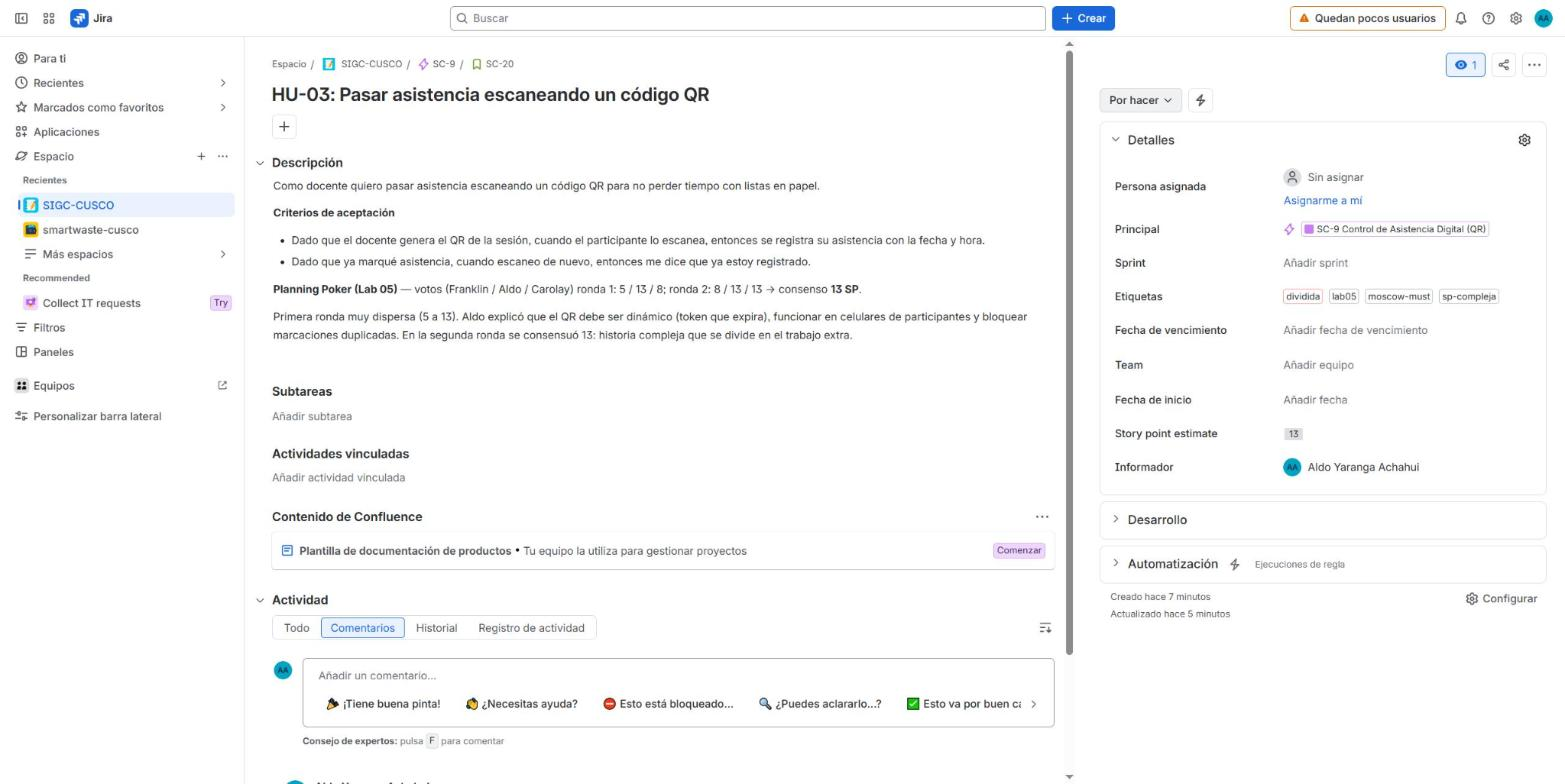
\includegraphics[width=\textwidth]{figura4_detalle_sc20_jira.jpg}
    \caption{Detalle de la historia SC-20 (HU-03) en Jira Software: votos de ambas rondas en la descripción, campo Story point estimate = 13 y etiquetas \texttt{sp-compleja}, \texttt{dividida}, \texttt{lab05} y \texttt{moscow-must}.}
    \label{fig:jira_detalle_sc20}
\end{figure}

\subsection{Clasificación de las Historias de Usuario por Tamaño}

De acuerdo con las directrices metodológicas de la guía de laboratorio, las historias de usuario fueron agrupadas en tres categorías según su puntaje de Fibonacci:
\begin{itemize}
    \item \textbf{Historias Cortas (1--3 SP):} Tareas atómicas de baja complejidad, con bajo riesgo y esfuerzo acotado (interfaces de consulta, notificaciones estándar o autenticación preconfigurada).
    \item \textbf{Historias Medias (5--8 SP):} Requerimientos que exigen lógica de negocio sustancial, transacciones con validación de integridad o reportería estructurada, pero cuya arquitectura es plenamente conocida por el equipo.
    \item \textbf{Historias Complejas (13+ SP):} Requerimientos de alta incertidumbre, dependencias externas críticas o arquitectura no trivial que no deben abordarse directamente en un sprint sin descomposición previa.
\end{itemize}

La Tabla~\ref{tab:clasificacion_historias} sintetiza el criterio de clasificación y la distribución estadística resultante en el backlog inicial del SIGC-CUSCO.

\begin{table}[H]
\centering
\small
\renewcommand{\arraystretch}{1.2}
\caption{Criterio de clasificación por tamaño y distribución estadística del backlog inicial.}
\label{tab:clasificacion_historias}
\begin{tabularx}{\textwidth}{P{2.2cm} C{2.2cm} C{2.2cm} C{2.0cm} Y}
\toprule
\rowcolor{headerblue}
\textcolor{white}{\textbf{Categoría}} & \textcolor{white}{\textbf{Rango}} & \textcolor{white}{\textbf{N° Historias}} & \textcolor{white}{\textbf{Suma SP}} & \textcolor{white}{\textbf{Historias Incluidas}} \\
\midrule
\rowcolor{white}
\textbf{Cortas} & 1--3 SP & 4 (30.8\%) & 11 SP (11.1\%) & HU-02, HU-08, HU-12, HU-13 \\
\rowcolor{rowalt}
\textbf{Medias} & 5--8 SP & 5 (38.5\%) & 28 SP (28.3\%) & HU-01, HU-04, HU-06, HU-09, HU-10 \\
\rowcolor{white}
\textbf{Complejas} & 13+ SP & 4 (30.8\%) & 60 SP (60.6\%) & HU-03, HU-05, HU-07, HU-11 \\
\midrule
\rowcolor{headerblue!10}
\textbf{Total Inicial} & -- & \textbf{13 historias} & \textbf{99 SP} & \textit{Concentración del 60.6\% del esfuerzo en complejas} \\
\bottomrule
\end{tabularx}
\end{table}

\textbf{Diagnóstico analítico de la distribución:}
El resultado inicial revela un síntoma clásico en la gestión de proyectos de software: aunque las historias complejas representan únicamente el $30.8\%$ del número de ítems (4 de 13), concentran más del \textbf{60\% del esfuerzo total del backlog} (60 de 99 SP). Introducir estas cuatro historias en su estado actual dentro de los sprints de desarrollo provocaría cuellos de botella en control de calidad, bloqueos imprevistos e incrementos de deuda técnica. Esta evidencia cuantitativa confirma la necesidad imperativa del refinamiento abordado en el trabajo extra.

\subsection{Entregable Oficial: Product Backlog con Estimaciones}

La Tabla~\ref{tab:product_backlog_estimado} presenta el Product Backlog formal del SIGC-CUSCO, ordenado estratégicamente por nivel de prioridad MoSCoW, integrando la clave Jira, código de historia, título descriptivo, épica, prioridad, valor en Story Points y su clasificación cualitativa.

\begin{table}[H]
\centering
\small
\renewcommand{\arraystretch}{1.18}
\caption{Product Backlog estimado del SIGC-CUSCO ordenado por prioridad MoSCoW.}
\label{tab:product_backlog_estimado}
\begin{tabularx}{\textwidth}{P{1.2cm} P{1.2cm} Y P{3.2cm} C{2.2cm} C{1.2cm} C{2.4cm}}
\toprule
\rowcolor{headerblue}
\textcolor{white}{\textbf{Clave}} & \textcolor{white}{\textbf{Código}} & \textcolor{white}{\textbf{Historia de Usuario}} & \textcolor{white}{\textbf{Épica}} & \textcolor{white}{\textbf{Prioridad}} & \textcolor{white}{\textbf{SP}} & \textcolor{white}{\textbf{Tipo}} \\
\midrule
\rowcolor{white}
SC-13 & HU-10 & Asignar roles a los usuarios para controlar acceso & Multientidad & Highest / Must & 5 & \badgeMedia \\
\rowcolor{rowalt}
SC-16 & HU-06 & Crear capacitaciones con fechas y cupos & Catálogo/Inscrip. & Highest / Must & 5 & \badgeMedia \\
\rowcolor{white}
SC-19 & HU-01 & Inscribirme a una capacitación usando DNI & Catálogo/Inscrip. & Highest / Must & 8 & \badgeMedia \\
\rowcolor{rowalt}
SC-20 & HU-03 & Pasar asistencia escaneando código QR & Asistencia QR & High / Must & 13 & \badgeCompleja \\
\rowcolor{white}
SC-21 & HU-04 & Registrar notas y calcular aprobación automát. & Evaluación & High / Must & 5 & \badgeMedia \\
\rowcolor{rowalt}
SC-22 & HU-05 & Generar y descargar certificado PDF con QR & Certificados & High / Must & 13 & \badgeCompleja \\
\rowcolor{white}
SC-14 & HU-07 & Registrar diferentes instituciones en el sistema & Multientidad & Medium / Should & 13 & \badgeCompleja \\
\rowcolor{rowalt}
SC-23 & HU-08 & Verificar autenticidad de certificado mediante QR & Certificados & Medium / Should & 3 & \badgeCorta \\
\rowcolor{white}
SC-24 & HU-09 & Generar reportes de cursos para auditorías & Reportes/Notif. & Medium / Should & 5 & \badgeMedia \\
\rowcolor{rowalt}
SC-25 & HU-02 & Recibir correo de confirmación al inscribirme & Reportes/Notif. & Medium / Should & 2 & \badgeCorta \\
\rowcolor{white}
SC-18 & HU-13 & Iniciar sesión con DNI y recuperar contraseña & Multientidad & Medium / Should & 3 & \badgeCorta \\
\rowcolor{rowalt}
SC-26 & HU-12 & Consultar catálogo público de cursos disponibles & Catálogo/Inscrip. & Low / Could & 3 & \badgeCorta \\
\rowcolor{white}
SC-27 & HU-11 & Marcar asistencia en modo offline con sincro. & Asistencia QR & Low / Could & 21 & \badgeCompleja \\
\bottomrule
\end{tabularx}
\end{table}

La Figura~\ref{fig:backlog_clasificado} complementa este entregable exhibiendo la distribución gráfica de los 99 Story Points y la jerarquía de tamaños obtenida en el sistema Jira.

\begin{figure}[H]
    \centering
    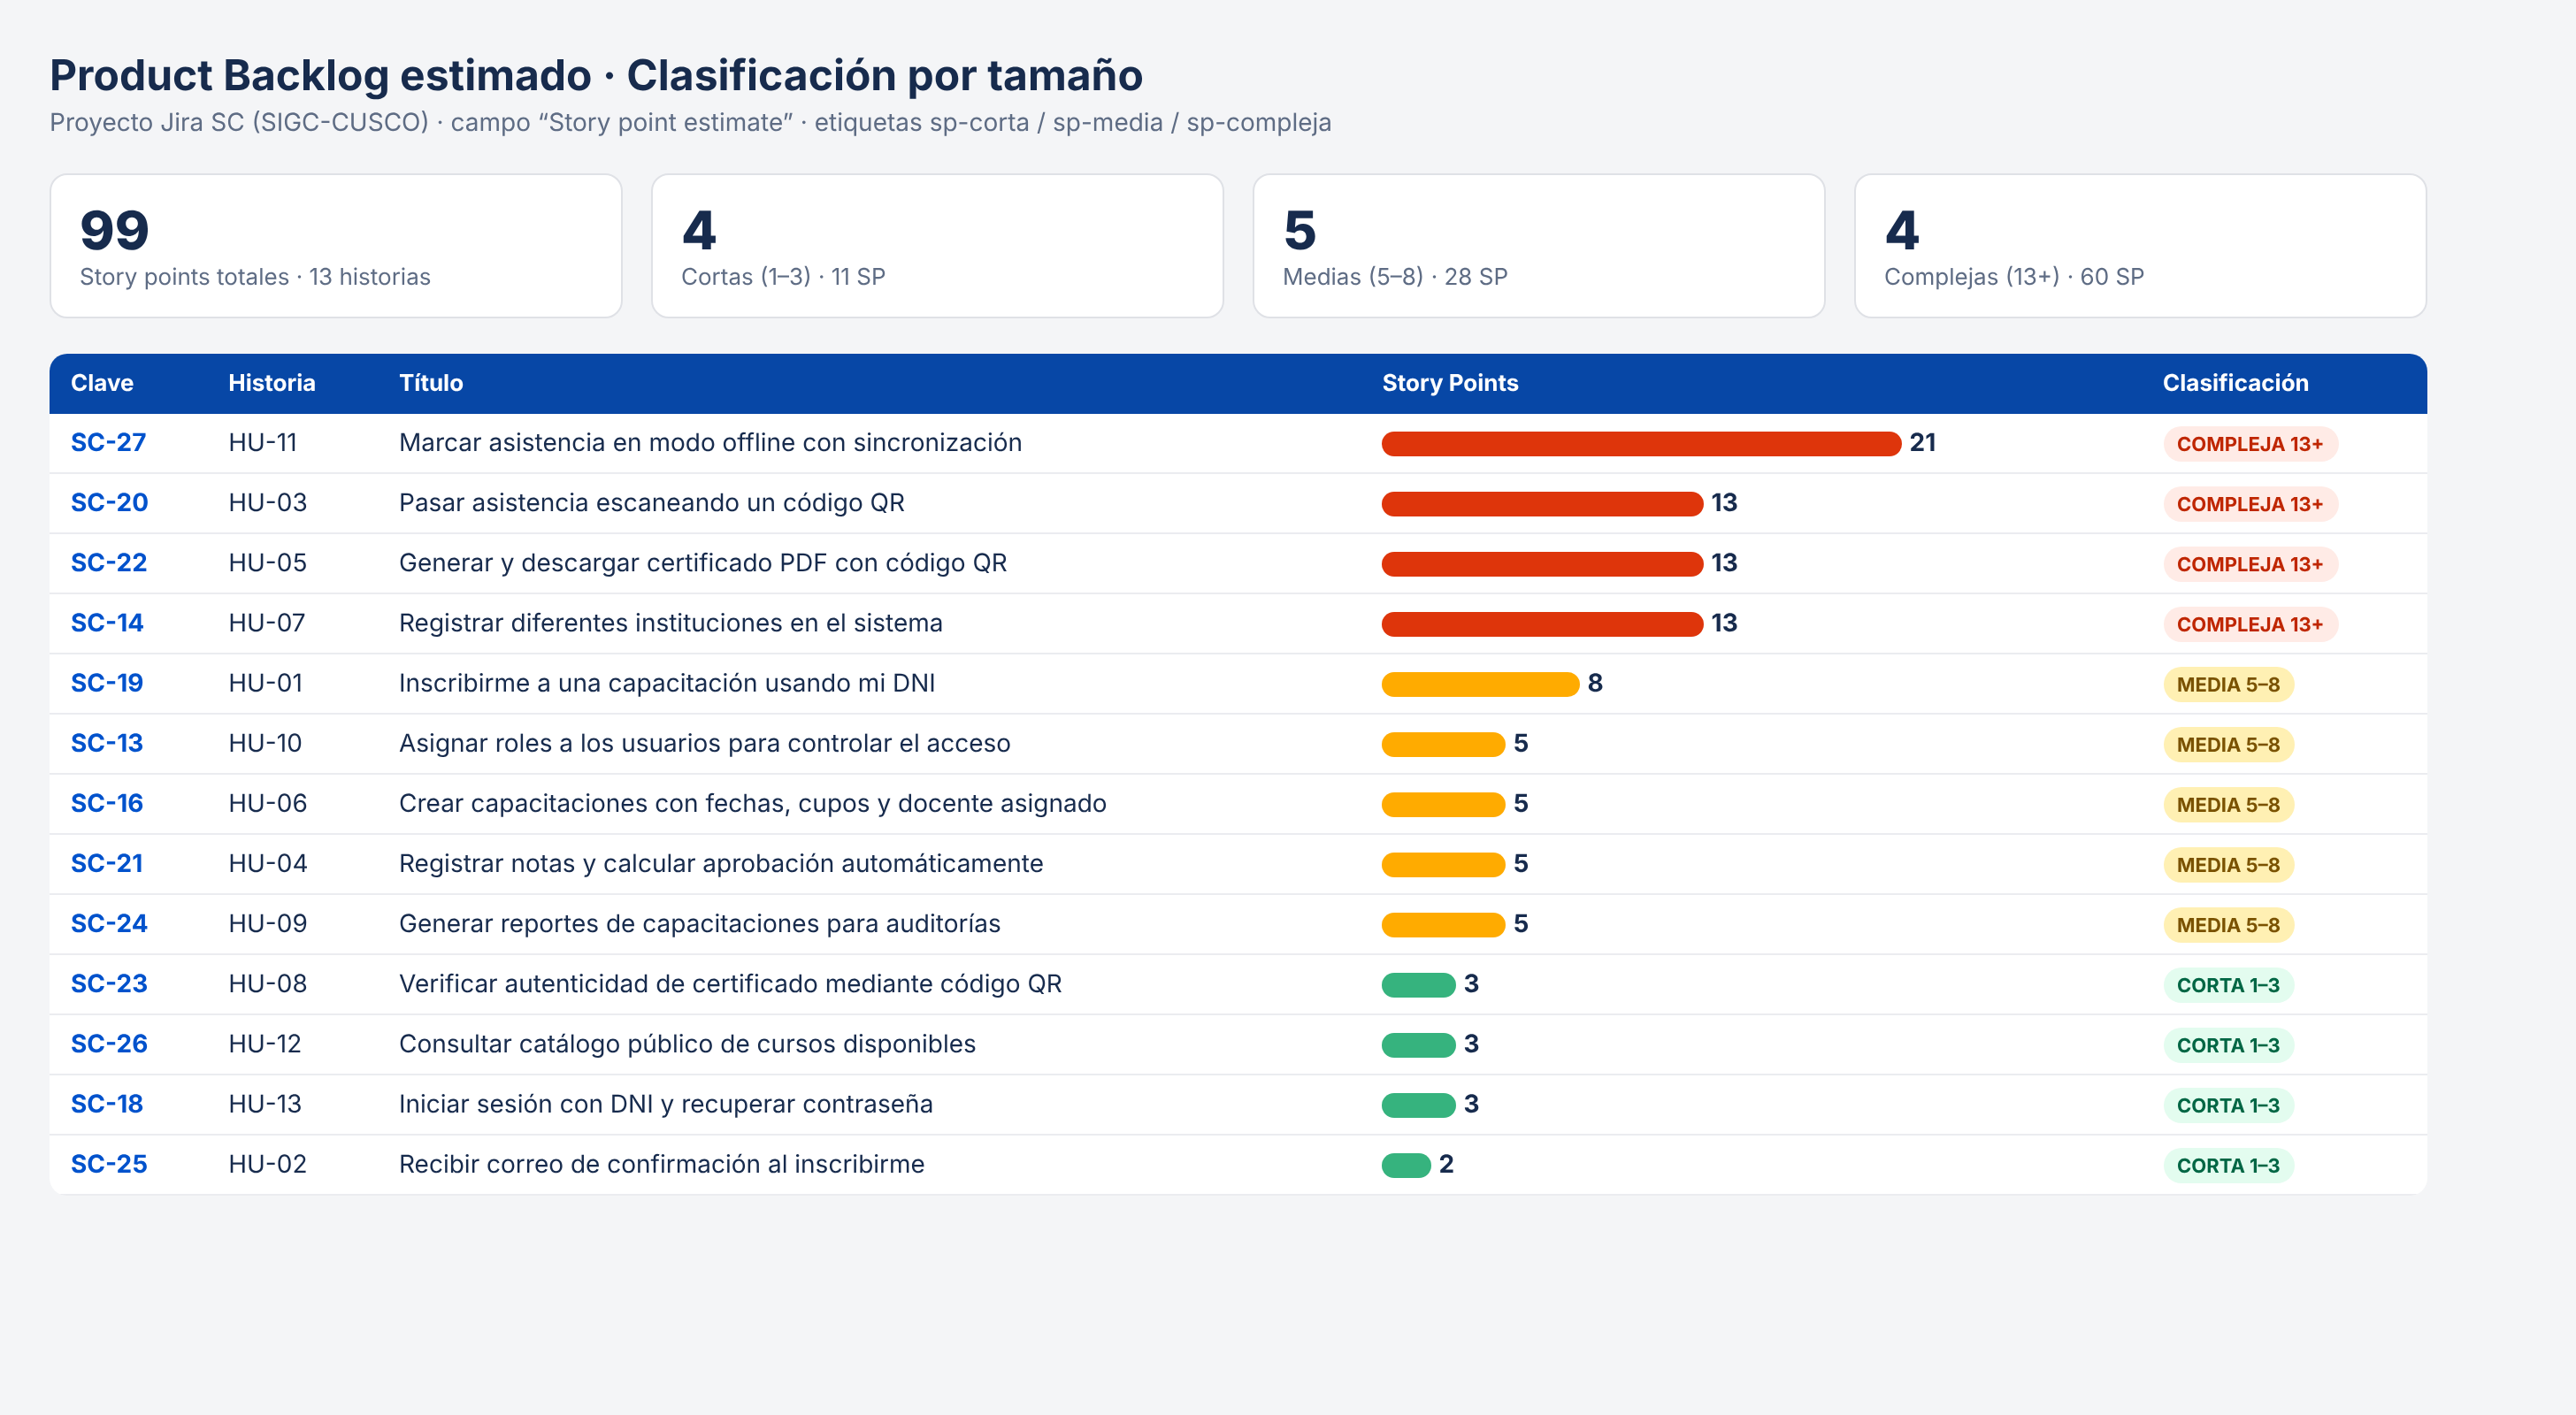
\includegraphics[width=\textwidth]{figura5_backlog_clasificado.png}
    \caption{Visualización ejecutiva del Product Backlog estimado y clasificado por tamaño (Proyecto SC en Jira).}
    \label{fig:backlog_clasificado}
\end{figure}

\subsection{Lectura Analítica y Estrategia de Planificación del Sprint 1}

Una lectura reflexiva de las estimaciones arroja pautas operativas fundamentales para el desarrollo del proyecto:
\begin{enumerate}
    \item \textbf{Carga del núcleo crítico (Must Have):} Las historias clasificadas como \textit{Must Have} totalizan \textbf{49 Story Points}. De ellas, cuatro corresponden a funcionalidades medias (HU-10, HU-06, HU-01 y HU-04, que suman 23 SP), mientras que dos son historias complejas sobredimensionadas (HU-03 y HU-05, sumando 26 SP).
    \item \textbf{Estrategia de ejecución para el Sprint 1:} Sería un error crítico iniciar el desarrollo atacando de golpe las historias de 13 SP. La estrategia idónea consiste en concentrar el primer incremento (Sprint 1) en las historias medias y cortas de cimiento: autenticación y roles (\texttt{HU-13}, \texttt{HU-10}), creación de cursos (\texttt{HU-06}) y el catálogo público con inscripción básica (\texttt{HU-12}, \texttt{HU-01}). Esto permite entregar un sistema funcional de registro mientras en paralelo se refinan y prototipan los componentes de asistencia QR y certificación digital.
    \item \textbf{Disponibilidad de artefactos:} El Product Backlog estimado se encuentra versionado formalmente en el repositorio GitHub en el archivo \texttt{backlog/product\_backlog\_estimado.csv}, garantizando su interoperabilidad con herramientas de reporting automatizado.
\end{enumerate}

\vspace{0.3cm}

% 7. Trabajo Extra: Refinamiento de Historias Grandes
\section{Trabajo Extra: Refinamiento de Historias Grandes}

\subsection{Criterios y Justificación de la Descomposición Ágil}

En el desarrollo de software ágil, una historia de usuario valorada en 13 o 21 Story Points constituye un \textbf{antipatrón} para la planificación de sprints por múltiples razones:
\begin{enumerate}
    \item \textbf{Violación del principio INVEST (\textit{Small}):} Una historia de 13 o 21 puntos excede con creces la capacidad de absorción y el margen de seguridad de una iteración estándar de dos semanas en un equipo universitario.
    \item \textbf{Efecto binario \enquote{Todo o Nada}:} Si un requerimiento masivo se traba en su fase final de pruebas o despliegue, la historia completa pasa al siguiente sprint con 0 puntos entregados, arruinando la predictibilidad de la velocidad del equipo.
    \item \textbf{Incertidumbre enmascarada:} Los puntajes elevados suelen ser un síntoma de que el requerimiento es en realidad una \textbf{Épica camuflada} que engloba flujos alternativos, reglas de negocio no analizadas y riesgos de integración no dimensionados.
\end{enumerate}

Para corregir esta situación, el equipo sometió las cuatro historias complejas (\texttt{HU-03}, \texttt{HU-05}, \texttt{HU-07} y \texttt{HU-11}) a un proceso formal de refinamiento (*Backlog Refinement*), aplicando patrones de división reconocidos en la industria (marco SPIDR y división por reglas de negocio/flujos):

\begin{itemize}
    \item \textbf{División por rol y secuencia del flujo (\texttt{HU-03}):} La marcación de asistencia QR involucra dos actores con necesidades asimétricas. Se descompuso en lo que compete al docente (generación del código QR dinámico proyectado), lo que compete al participante (escaneo y validación desde la cámara web/móvil) y la capa de control antifraude (bloqueo de duplicados y visualización de la nómina de presentes en tiempo real).
    \item \textbf{División por reglas de negocio y valor incremental (\texttt{HU-05}):} La emisión de certificados se fragmentó desacoplando la lógica de validación previa (cálculo de notas y umbral de asistencia), la renderización física del PDF vectorial con firma y hash SHA-256 para un alumno individual, y el subsistema de procesamiento por lotes (*batch job*) para emitir masivamente todos los diplomas de un curso al término del acta.
    \item \textbf{División por capas de valor y alcance operativo (\texttt{HU-07}):} En la gestión multientidad se independizó la creación básica de la entidad institucional (datos fiscales y logo), la asociación relacional de usuarios y capacitaciones a dicha entidad, y la implementación rigurosa de los filtros globales de aislamiento de datos en las consultas Eloquent.
    \item \textbf{Técnica del Spike Técnico con tiempo delimitado (\texttt{HU-11}):} Dado que el modo offline representaba una barrera tecnológica desconocida para el equipo, se aisló en primera instancia un \textbf{Spike de Investigación (2 SP)}. Este spike no busca entregar código productivo, sino un prototipo descartable para evaluar la viabilidad de la API de \textit{Service Workers} e \textit{IndexedDB}. Una vez desarmada la incertidumbre, el almacenamiento local, la sincronización en segundo plano y los indicadores visuales pudieron dimensionarse con total confianza.
\end{itemize}

Cada historia hija resultante fue formulada manteniendo la sintaxis estándar \textit{Como / Quiero / Para}, provista de criterios de aceptación propios y re-estimada en equipo bajo la misma baraja de Fibonacci.

\subsection{Historias Refinadas y Re-estimación en Jira}

La Tabla~\ref{tab:historias_refinadas} detalla la correspondencia entre las cuatro historias padre originales, sus historias hijas creadas en Jira Software (claves \texttt{SC-28} a \texttt{SC-40}), los nuevos puntajes de Story Points asignados y su clasificación.

\begin{table}[H]
\centering
\small
\renewcommand{\arraystretch}{1.18}
\caption{Matriz de refinamiento y re-estimación de las historias complejas (etiquetadas como \texttt{refinamiento} en Jira).}
\label{tab:historias_refinadas}
\begin{tabularx}{\textwidth}{P{1.2cm} P{2.0cm} P{1.2cm} P{1.4cm} Y C{1.2cm} C{2.2cm}}
\toprule
\rowcolor{headerblue}
\textcolor{white}{\textbf{Clave}} & \textcolor{white}{\textbf{Origen (SP)}} & \textcolor{white}{\textbf{Nueva}} & \textcolor{white}{\textbf{Código}} & \textcolor{white}{\textbf{Historia de Usuario Refinada}} & \textcolor{white}{\textbf{SP}} & \textcolor{white}{\textbf{Tipo}} \\
\midrule
\rowcolor{white}
\textbf{SC-14} & \textbf{HU-07} & SC-28 & HU-07.1 & Registrar institución con RUC, razón social y logo & 3 & \badgeCorta \\
\rowcolor{white}
& \textit{(13 SP)} & SC-29 & HU-07.2 & Asociar usuarios y capacitaciones a una institución & 5 & \badgeMedia \\
\rowcolor{white}
& & SC-30 & HU-07.3 & Aislar los datos para que cada institución vea lo suyo & 5 & \badgeMedia \\
\rowcolor{rowalt}
\multicolumn{5}{r}{\textbf{Subtotal refinado HU-07:}} & \textbf{13 SP} & \textit{3 historias} \\
\midrule
\rowcolor{white}
\textbf{SC-20} & \textbf{HU-03} & SC-31 & HU-03.1 & Generar QR dinámico por sesión (vista docente) & 5 & \badgeMedia \\
\rowcolor{white}
& \textit{(13 SP)} & SC-32 & HU-03.2 & Registrar asistencia escaneando el QR (participante) & 5 & \badgeMedia \\
\rowcolor{white}
& & SC-33 & HU-03.3 & Evitar marcaciones duplicadas y ver lista de sesión & 3 & \badgeCorta \\
\rowcolor{rowalt}
\multicolumn{5}{r}{\textbf{Subtotal refinado HU-03:}} & \textbf{13 SP} & \textit{3 historias} \\
\midrule
\rowcolor{white}
\textbf{SC-22} & \textbf{HU-05} & SC-34 & HU-05.1 & Validar requisitos de emisión (nota $\ge 11$ y asistencia) & 3 & \badgeCorta \\
\rowcolor{white}
& \textit{(13 SP)} & SC-35 & HU-05.2 & Generar PDF con plantilla, QR vectorial y hash SHA-256 & 5 & \badgeMedia \\
\rowcolor{white}
& & SC-36 & HU-05.3 & Emitir certificados en lote para todo un curso & 5 & \badgeMedia \\
\rowcolor{rowalt}
\multicolumn{5}{r}{\textbf{Subtotal refinado HU-05:}} & \textbf{13 SP} & \textit{3 historias} \\
\midrule
\rowcolor{white}
\textbf{SC-27} & \textbf{HU-11} & SC-37 & HU-11.1 & Spike: evaluar almacenamiento local (PWA + IndexedDB) & 2 & \badgeCorta \\
\rowcolor{white}
& \textit{(21 SP)} & SC-38 & HU-11.2 & Guardar asistencias en el dispositivo en modo offline & 5 & \badgeMedia \\
\rowcolor{white}
& & SC-39 & HU-11.3 & Sincronizar asistencias pendientes al reconectar sin duplicados & 8 & \badgeMedia \\
\rowcolor{white}
& & SC-40 & HU-11.4 & Mostrar indicador visual de datos pendientes de sincronizar & 3 & \badgeCorta \\
\rowcolor{rowalt}
\multicolumn{5}{r}{\textbf{Subtotal refinado HU-11:}} & \textbf{18 SP} & \textit{4 historias} \\
\midrule
\rowcolor{headerblue!10}
\multicolumn{5}{r}{\textbf{Total Refinado (13 historias hijas):}} & \textbf{57 SP} & \textit{Reducción de riesgo} \\
\bottomrule
\end{tabularx}
\end{table}

La Figura~\ref{fig:refinamiento_historias} sintetiza visualmente este desglose estructural, mostrando cómo cada historia original compleja fue desmembrada y re-estimada en Jira.

\begin{figure}[H]
    \centering
    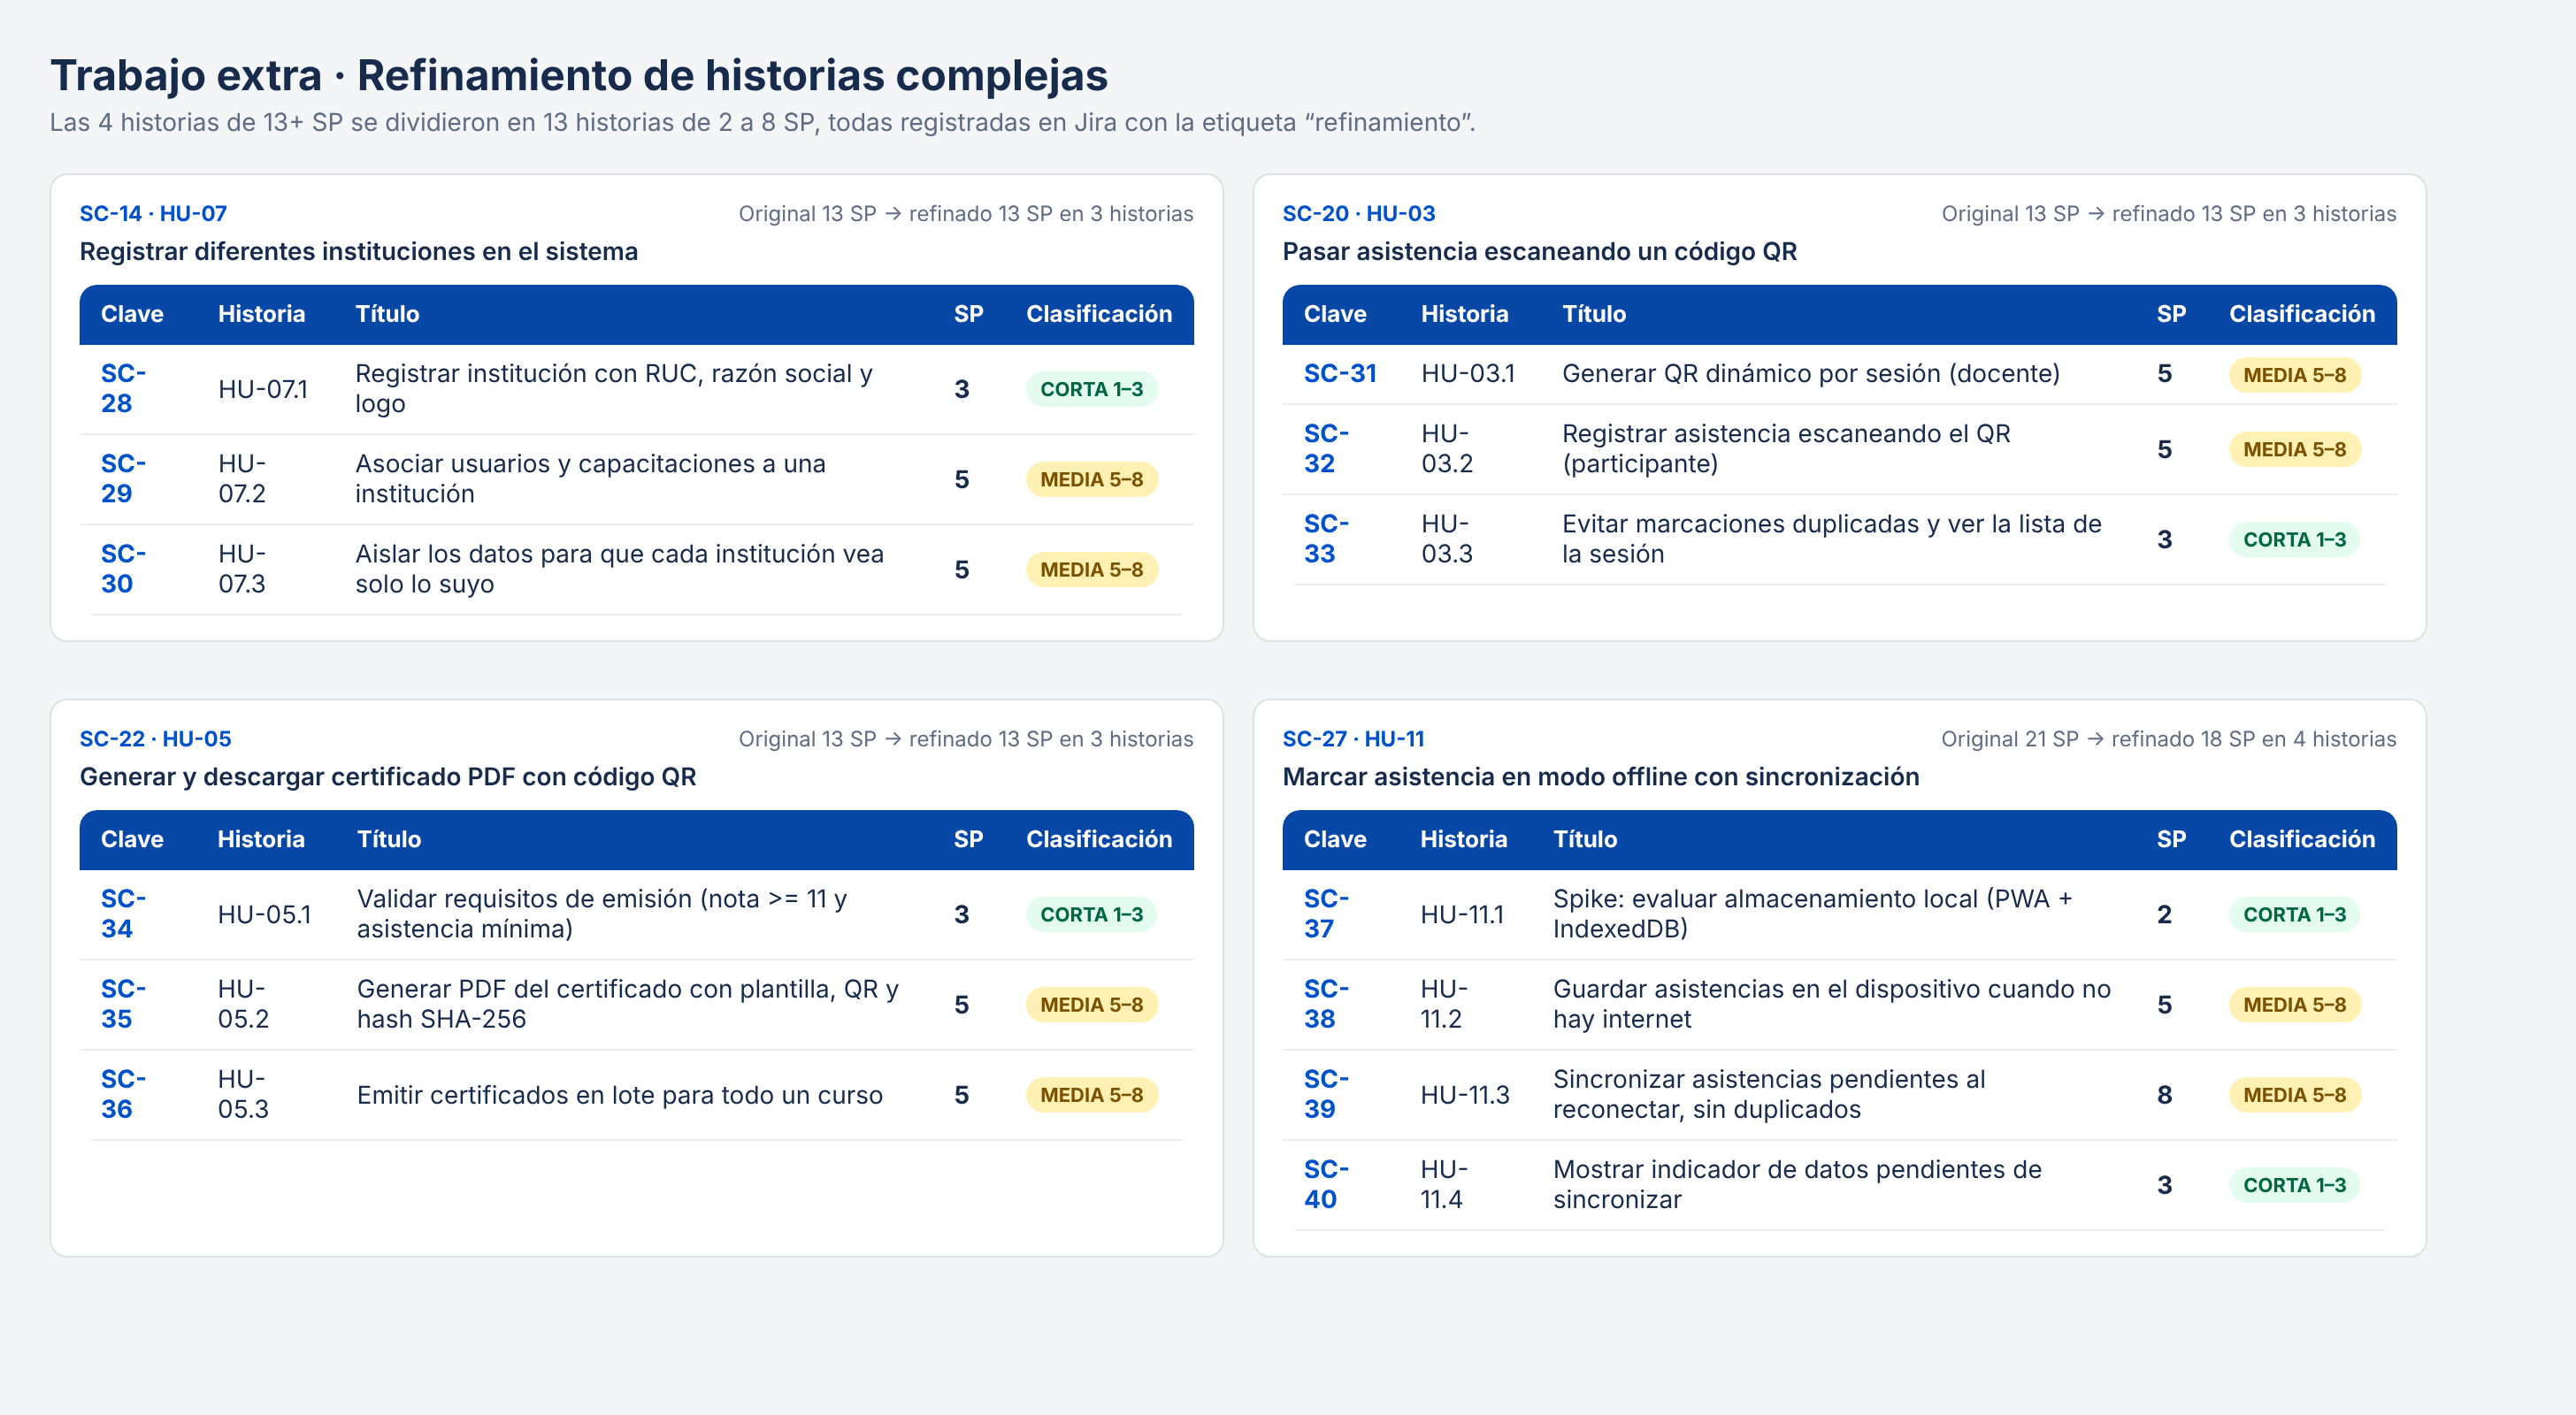
\includegraphics[width=\textwidth]{figura6_refinamiento_historias.png}
    \caption{Evidencia gráfica del trabajo extra: descomposición de las cuatro historias complejas de 13+ SP en 13 historias atómicas de 2 a 8 SP, con sus respectivas claves Jira y puntajes.}
    \label{fig:refinamiento_historias}
\end{figure}

\subsection{Impacto Cuantitativo y Cualitativo del Refinamiento}

El ejercicio de refinamiento generó un impacto positivo inmediato en la salud del Product Backlog:

\begin{enumerate}
    \item \textbf{Eliminación absoluta de historias no planificables:} Las 4 historias complejas (que sumaban 60 SP de alto riesgo) se convirtieron en 13 historias manejables que oscilan entre 2 y 8 SP. \textbf{En el backlog activo del SIGC-CUSCO ya no existe ninguna historia que supere los 8 Story Points}. Todas caben holgadamente dentro de una iteración y pueden ser probadas de manera autónoma.
    
    \item \textbf{Ahorro y precisión mediante el Spike Técnico (\texttt{HU-11}):} El requerimiento de sincronización offline redujo su estimación total de \textbf{21 a 18 SP}. Al separar formalmente el spike técnico (\texttt{HU-11.1} con 2 SP), el equipo aisló la fase de experimentación y prueba de concepto; las tres historias de implementación subsiguientes se estimaron sobre certezas funcionales (guardado local con 5 SP, sincronización con 8 SP y semáforo visual con 3 SP), eliminando el colchón de incertidumbre que inflaba la historia original.
    
    \item \textbf{Composición final del Backlog Activo:} Al sustituir las 4 historias padre por sus 13 hijas, el backlog operativo queda constituido por \textbf{22 historias de usuario} (9 historias originales no complejas + 13 historias refinadas). El esfuerzo global activo se ajustó de 99 a \textbf{96 Story Points}:
    \begin{itemize}
        \item \textbf{Historias Cortas (1--3 SP):} 10 historias (26 SP, 27.1\% del backlog).
        \item \textbf{Historias Medias (5--8 SP):} 12 historias (70 SP, 72.9\% del backlog).
        \item \textbf{Historias Complejas (13+ SP):} \textbf{0 historias activas} (0\%).
    \end{itemize}
    
    \item \textbf{Política de trazabilidad en Jira:} Las cuatro historias padre originales (\texttt{SC-14}, \texttt{SC-20}, \texttt{SC-22} y \texttt{SC-27}) se conservaron en Jira con el estado de cerradas por división, etiquetadas como \texttt{dividida} y vinculadas con enlaces de issue (\textit{\enquote{is parent of}}) hacia sus respectivas hijas. Esto preserva el historial de la estimación original como evidencia académica y de auditoría de procesos.
\end{enumerate}

\vspace{0.3cm}

% 8. Conclusiones y Lecciones Aprendidas
\section{Conclusiones y Lecciones Aprendidas}

A partir de la ejecución integral de las actividades del Laboratorio N° 05, el equipo de desarrollo formula las siguientes conclusiones académicas y lecciones aprendidas:

\begin{enumerate}
    \item \textbf{Efectividad del consenso mediante Planning Poker:} La técnica demostró ser significativamente superior a la estimación empírica en horas o a la asignación arbitraria por parte de un solo integrante. La votación secreta y la revelación simultánea anularon eficazmente el \textit{efecto de anclaje} y la presión jerárquica. El debate obligatorio entre los votos extremos (el más alto y el más bajo) enriqueció el entendimiento colectivo del sistema, unificando criterios sobre la arquitectura tecnológica a utilizar en el SIGC-CUSCO (uso de \textit{Policies} de Laravel, transacciones para control de cupos y generación vectorial de certificados).
    
    \item \textbf{La dispersión de votos como indicador temprano de riesgo técnico:} Se evidenció de forma empírica que la disparidad en la escala de Fibonacci no representa un fallo en la sesión, sino un \textbf{sensor precoz de incertidumbre o ambigüedad}. Coincidentemente, las únicas tres historias donde hubo divergencias profundas (\texttt{HU-03}, \texttt{HU-07} y \texttt{HU-11}) fueron aquellas con mayor desafío de seguridad o infraestructura (código QR dinámico TOTP, aislamiento multientidad por \textit{Global Scopes} y sincronización bidireccional offline). La dispersión obligó al equipo a detenerse, dialogar y precisar el alcance antes de escribir una sola línea de código.
    
    \item \textbf{Gobernanza y trazabilidad cuantitativa en Jira Software:} La integración de las estimaciones en Jira mediante el campo \texttt{Story point estimate}, las etiquetas de clasificación (\texttt{sp-corta}, \texttt{sp-media}, \texttt{sp-compleja}) y la documentación de las rondas de votación dota al proyecto de una infraestructura de seguimiento profesional. El uso de filtros JQL permite identificar de inmediato requerimientos en riesgo y planificar la velocidad del equipo con fundamentos numéricos reales.
    
    \item \textbf{Transformación de épicas ocultas mediante el Refinamiento:} El trabajo extra evidenció el peligro de mantener historias de 13 o 21 SP en el backlog activo: concentraban más del $60\%$ del esfuerzo total del proyecto y ponían en riesgo la entrega de los sprints. La descomposición en 13 historias hijas atómicas (de 2 a 8 SP) y el aislamiento de la investigación mediante un \textbf{Spike Técnico} en \texttt{HU-11} permitió reducir la incertidumbre, logrando un Product Backlog activo de \textbf{22 historias y 96 Story Points}, donde ningún ítem supera los 8 SP, maximizando la agilidad, la verificabilidad en pruebas y la capacidad de entrega continua.
\end{enumerate}


\end{document}
